\documentclass[14pt, table]{extarticle}
\usepackage{amsfonts}
\usepackage{amsmath}
\usepackage[utf8]{inputenc}
\usepackage[a4paper, total={7in, 10.5in}]{geometry}
\usepackage[table]{xcolor}
\usepackage{tgbonum}
\usepackage{float}
\usepackage{graphicx}
\graphicspath{ {./images/} }
\DeclareGraphicsExtensions{.png,.jpg}
\usepackage{caption}
\usepackage{tikz}
\usepackage{circuitikz}
\usepackage[T1]{fontenc}
\usetikzlibrary{quotes,angles}
\usetikzlibrary{arrows}
\hyphenpenalty 10000
\usepackage{subfig}
\usepackage{array}

\title{\textbf{Sprawozdanie} \\ \Large{Ćwiczenie 3}}
\date{Data wykonania: 19 kwietnia 2023}
\author{ \Large{Jan Kwinta} \\ \large{Prowadzący ćwiczenia: dr. Szymon Niedźwiedzki}}


\newcommand{\nl}{\vspace{0.5cm}}
\newcommand{\nz}{\vspace{1.5cm}}
\newcommand{\zatem}{\textrm{Zatem }}

\definecolor{trueGreen}{HTML}{009900}

\begin{document}
\maketitle

\paragraph{Wstęp \\}
Tematem trzecich zajęć z elektroniki były wzmacniacze operacyjne i układy elektryczne budowane przy ich użyciu: wzmacniacz odwracający fazę, sumator, przerzutnik Schmidta i multiwibrator astabilny. \\

Wzmacniacz odwracający fazę.

\begin{center}
\begin{circuitikz}

  	\draw (0, 0) node[op amp] (opamp) {};
	\draw (opamp.out) to [short,-o] +(2, 0);
	\draw (2, 0) to (2, 2.5)
			  to [european resistor=$R_f$] (-2, 2.5)
			  to (-2, 0.5); 
	
	\draw (opamp.-) to (-2, 0.5)
				to [european resistor=$R_1$] (-6, 0.5)
				to [short,-o] (-6.1, 0.5);

	\draw (opamp.+) to (-2, -0.5) 
				to (-2, -2) node[ground]{};

\end{circuitikz}
\end{center}

Sumator o dwóch wejściach.

\begin{center}
\begin{circuitikz}

  	\draw (0, 0) node[op amp] (opamp) {};
	\draw (opamp.out) to [short,-o] +(2, 0);
	\draw (2, 0) to (2, 2.5)
			  to [european resistor=$R_f$] (-2, 2.5)
			  to (-2, 0.5); 
	
	\draw (opamp.-) to (-2, 0.5)
				to (-3, 0.5)
				to [european resistor=$R_2$] (-7, 0.5)
				to [short,-o] (-7.1, 0.5);

	\draw (-3, 0.5) to (-3, 2)
				to [european resistor=$R_1$] (-7, 2)
				to [short,-o] (-7.1, 2);

	\draw (opamp.+) to (-2, -0.5) 
				to (-2, -2) node[ground]{};

\end{circuitikz}
\end{center}

Przerzutnik Schmidta.

\begin{center}
\begin{circuitikz}

  	\draw (0, 0) node[op amp] (opamp) {};
	\draw (opamp.out) to [short,-o] +(2, 0);

	\draw (2, 0) to [european resistor=$R_1$] (2, -2.5)
			  to [european resistor=$R_2$] (2, -5)
			  to (2, -5.1) node[ground]{}; 

	\draw (2, -2.5) to (-2, -2.5)
				to (-2, -0.5)
				to (opamp.+);

	\draw (opamp.-) to [short,-o] (-2, 0.5);

\end{circuitikz}
\end{center}

Multiwibrator astabilny.

\begin{center}
\begin{circuitikz}

  	\draw (0, 0) node[op amp] (opamp) {};
	\draw (opamp.out) to [short,-o] +(2, 0);

	\draw (2, 0) to (2, 2.5)
			  to [european resistor=$R_f$] (-2, 2.5)
			  to (-2, 0.5); 

	\draw (2, 0) to [european resistor=$R_1$] (2, -2.5)
			  to [european resistor=$R_2$] (2, -5)
			  to (2, -5.1) node[ground]{}; 

	\draw (2, -2.5) to (-2, -2.5)
				to (-2, -0.5)
				to (opamp.+);

	\draw (opamp.-) to (-2, 0.5)
				to (-4, 0.5)
				to [C=$C$] (-4, -3.1)
				to (-4, -5.1) node[ground]{};

\end{circuitikz}
\end{center}

\newpage
\paragraph{Ćwiczenie 3.1 \\}

Schemat ideowy wzmacniacza operacyjnego.

\begin{figure}[H]
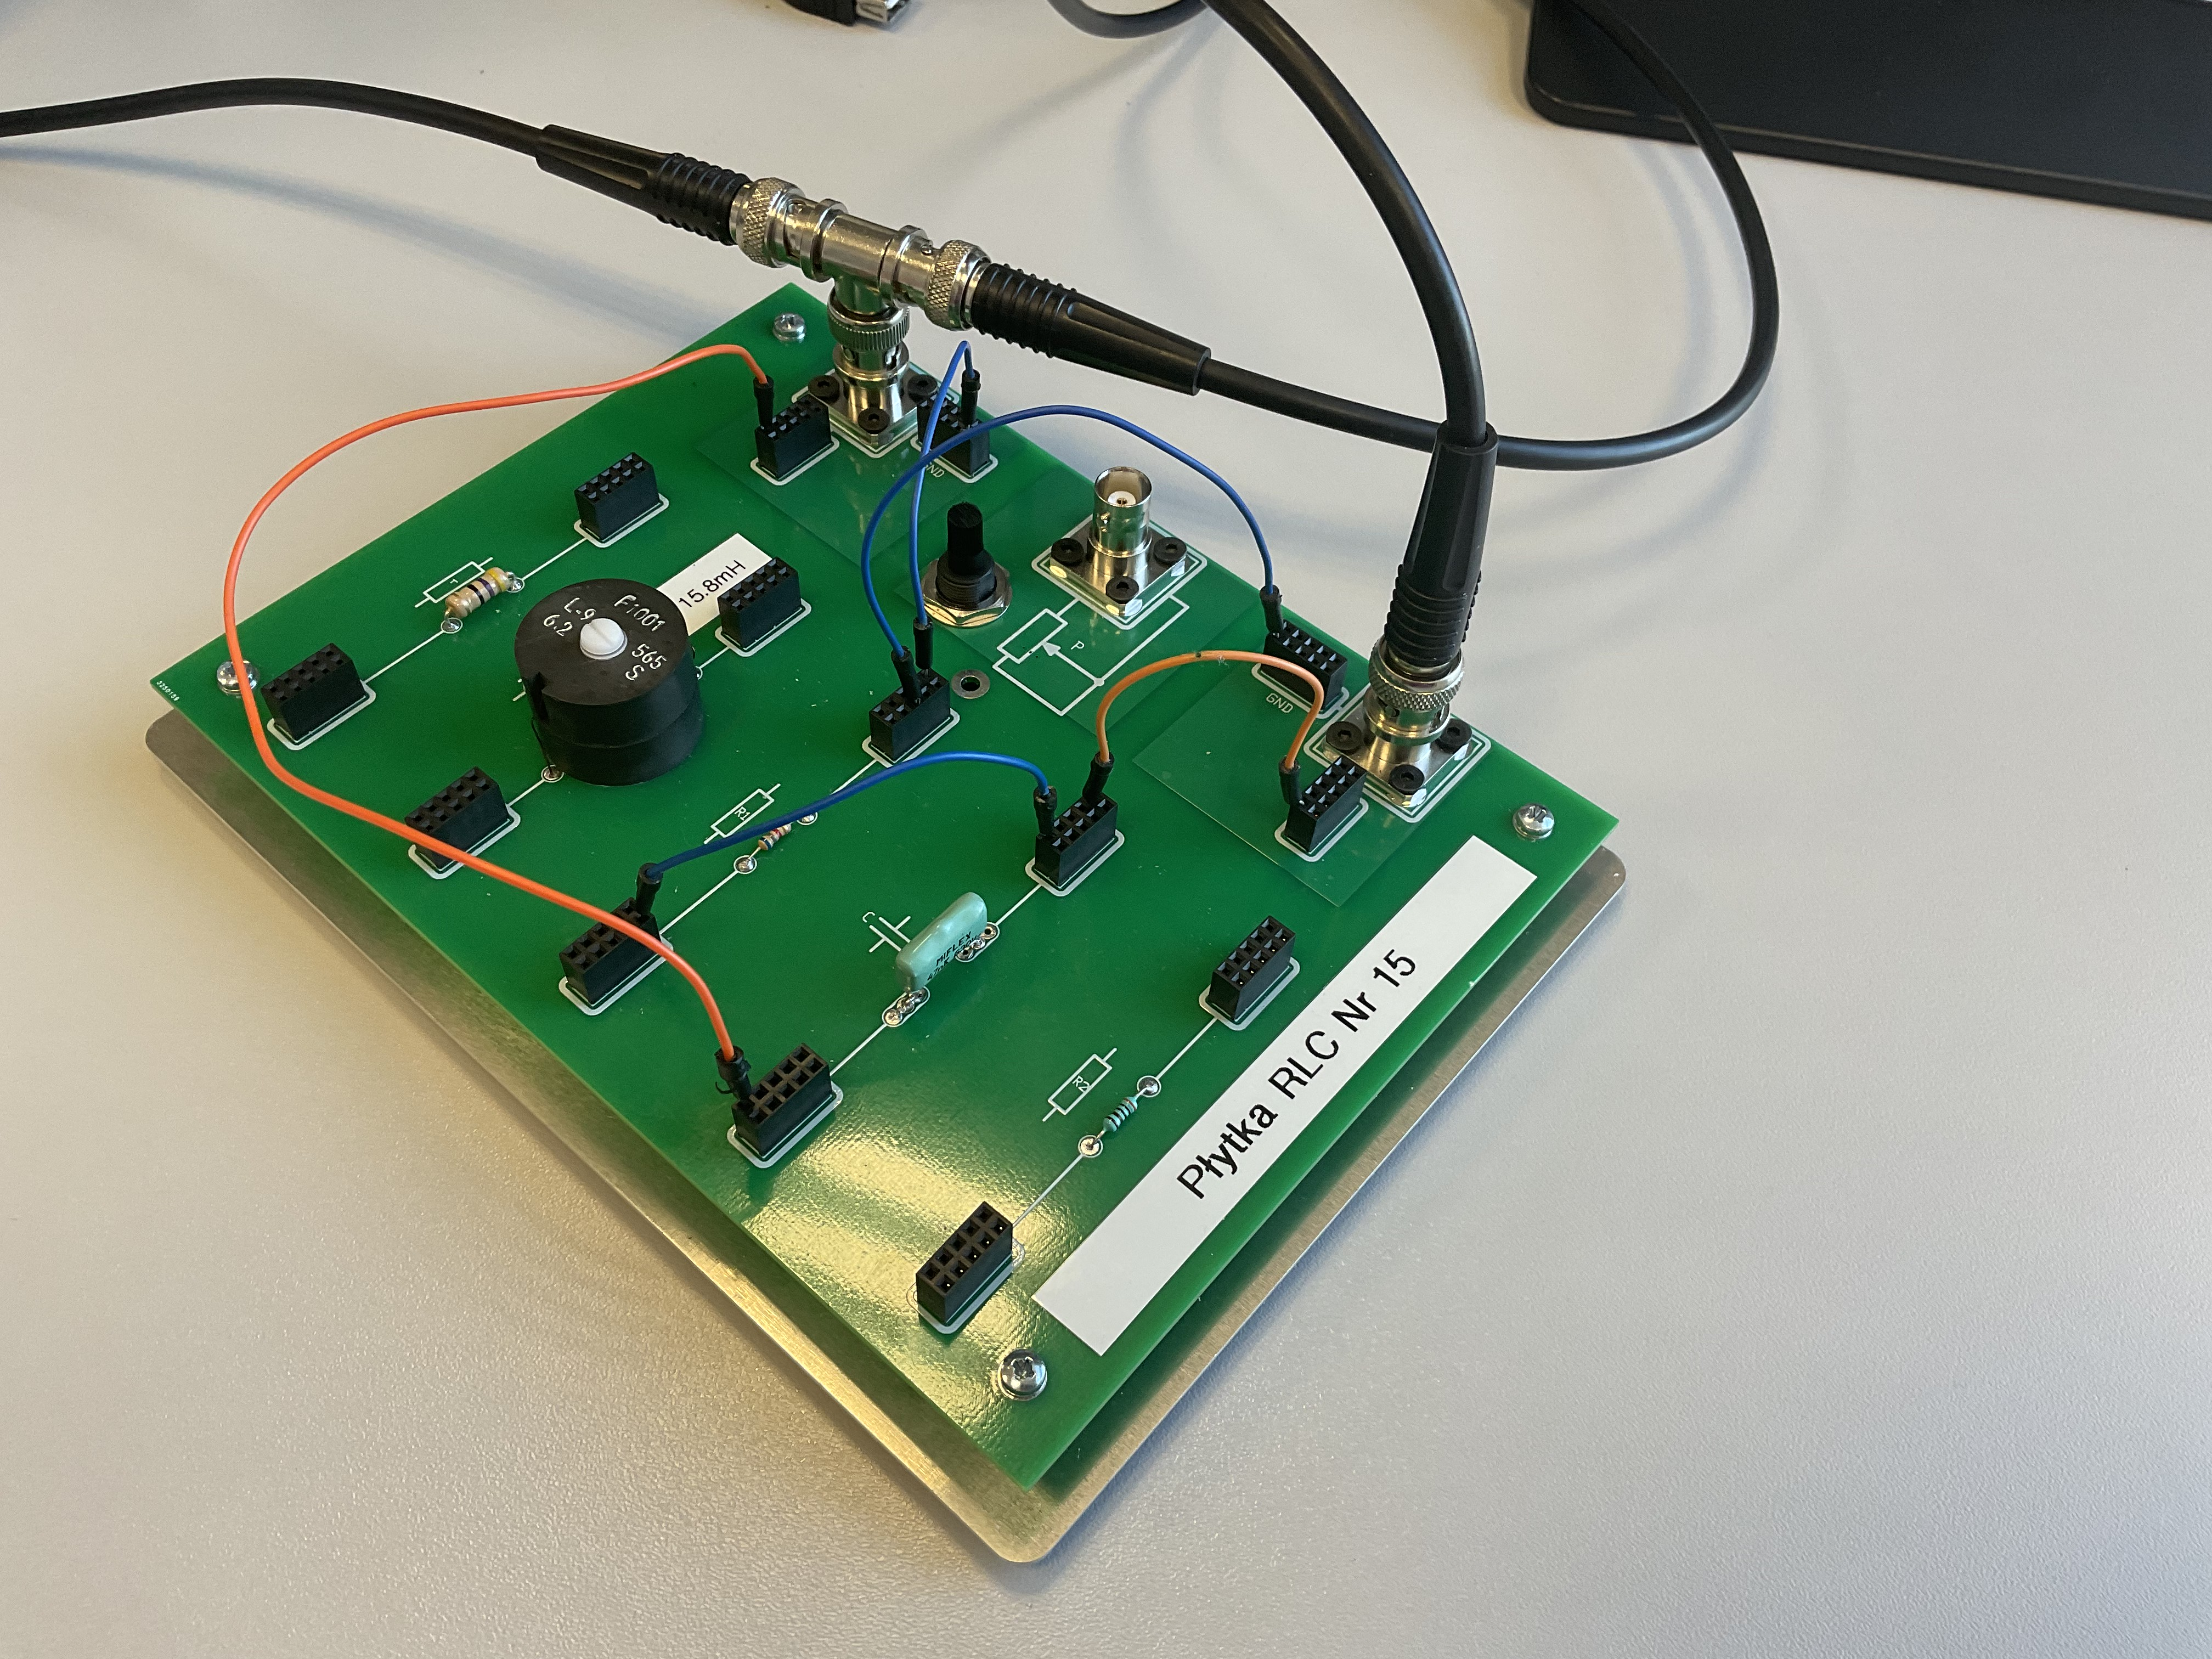
\includegraphics[scale=0.07]{C0}
\centering
\captionsetup{labelformat=empty}
\caption{Płytka ze wzmacniaczem operacyjnym.}
\end{figure}

\begin{figure}[H]
    \centering
    \subfloat[\centering Napięcie $12 \ V$]{{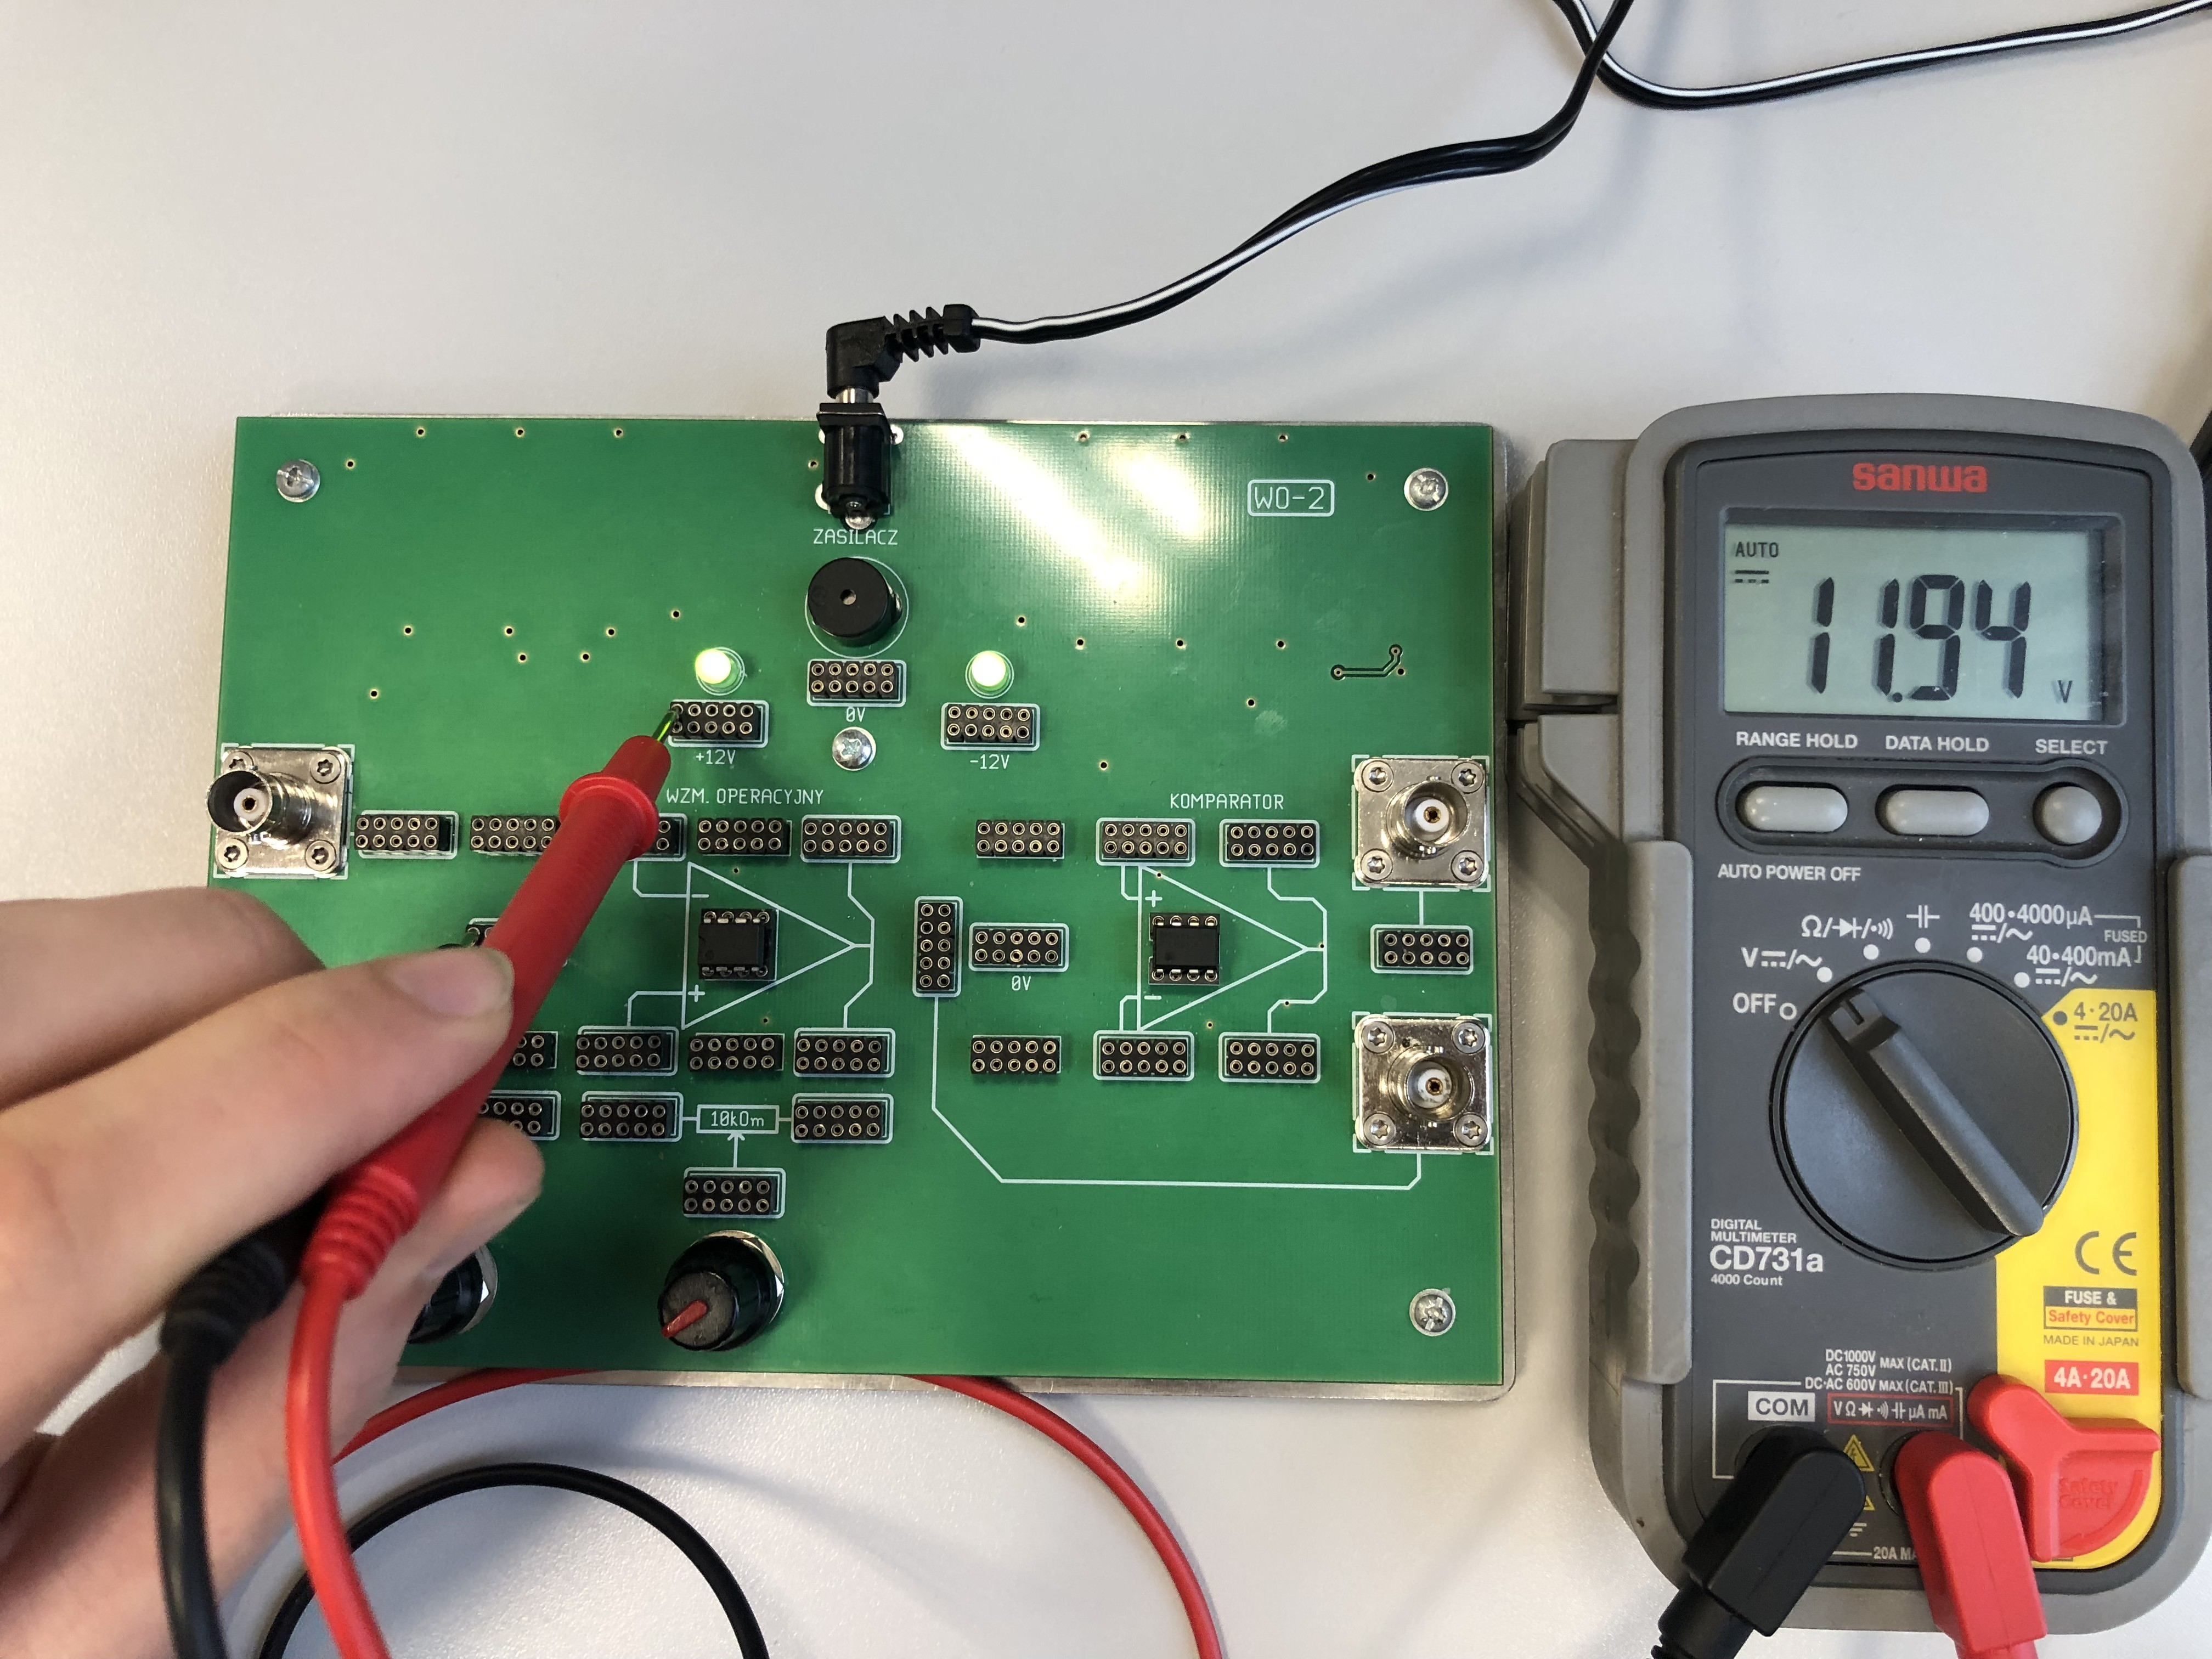
\includegraphics[width=7cm]{C8}}}%
    \qquad
    \subfloat[\centering Napięcie $-12 \ V$]{{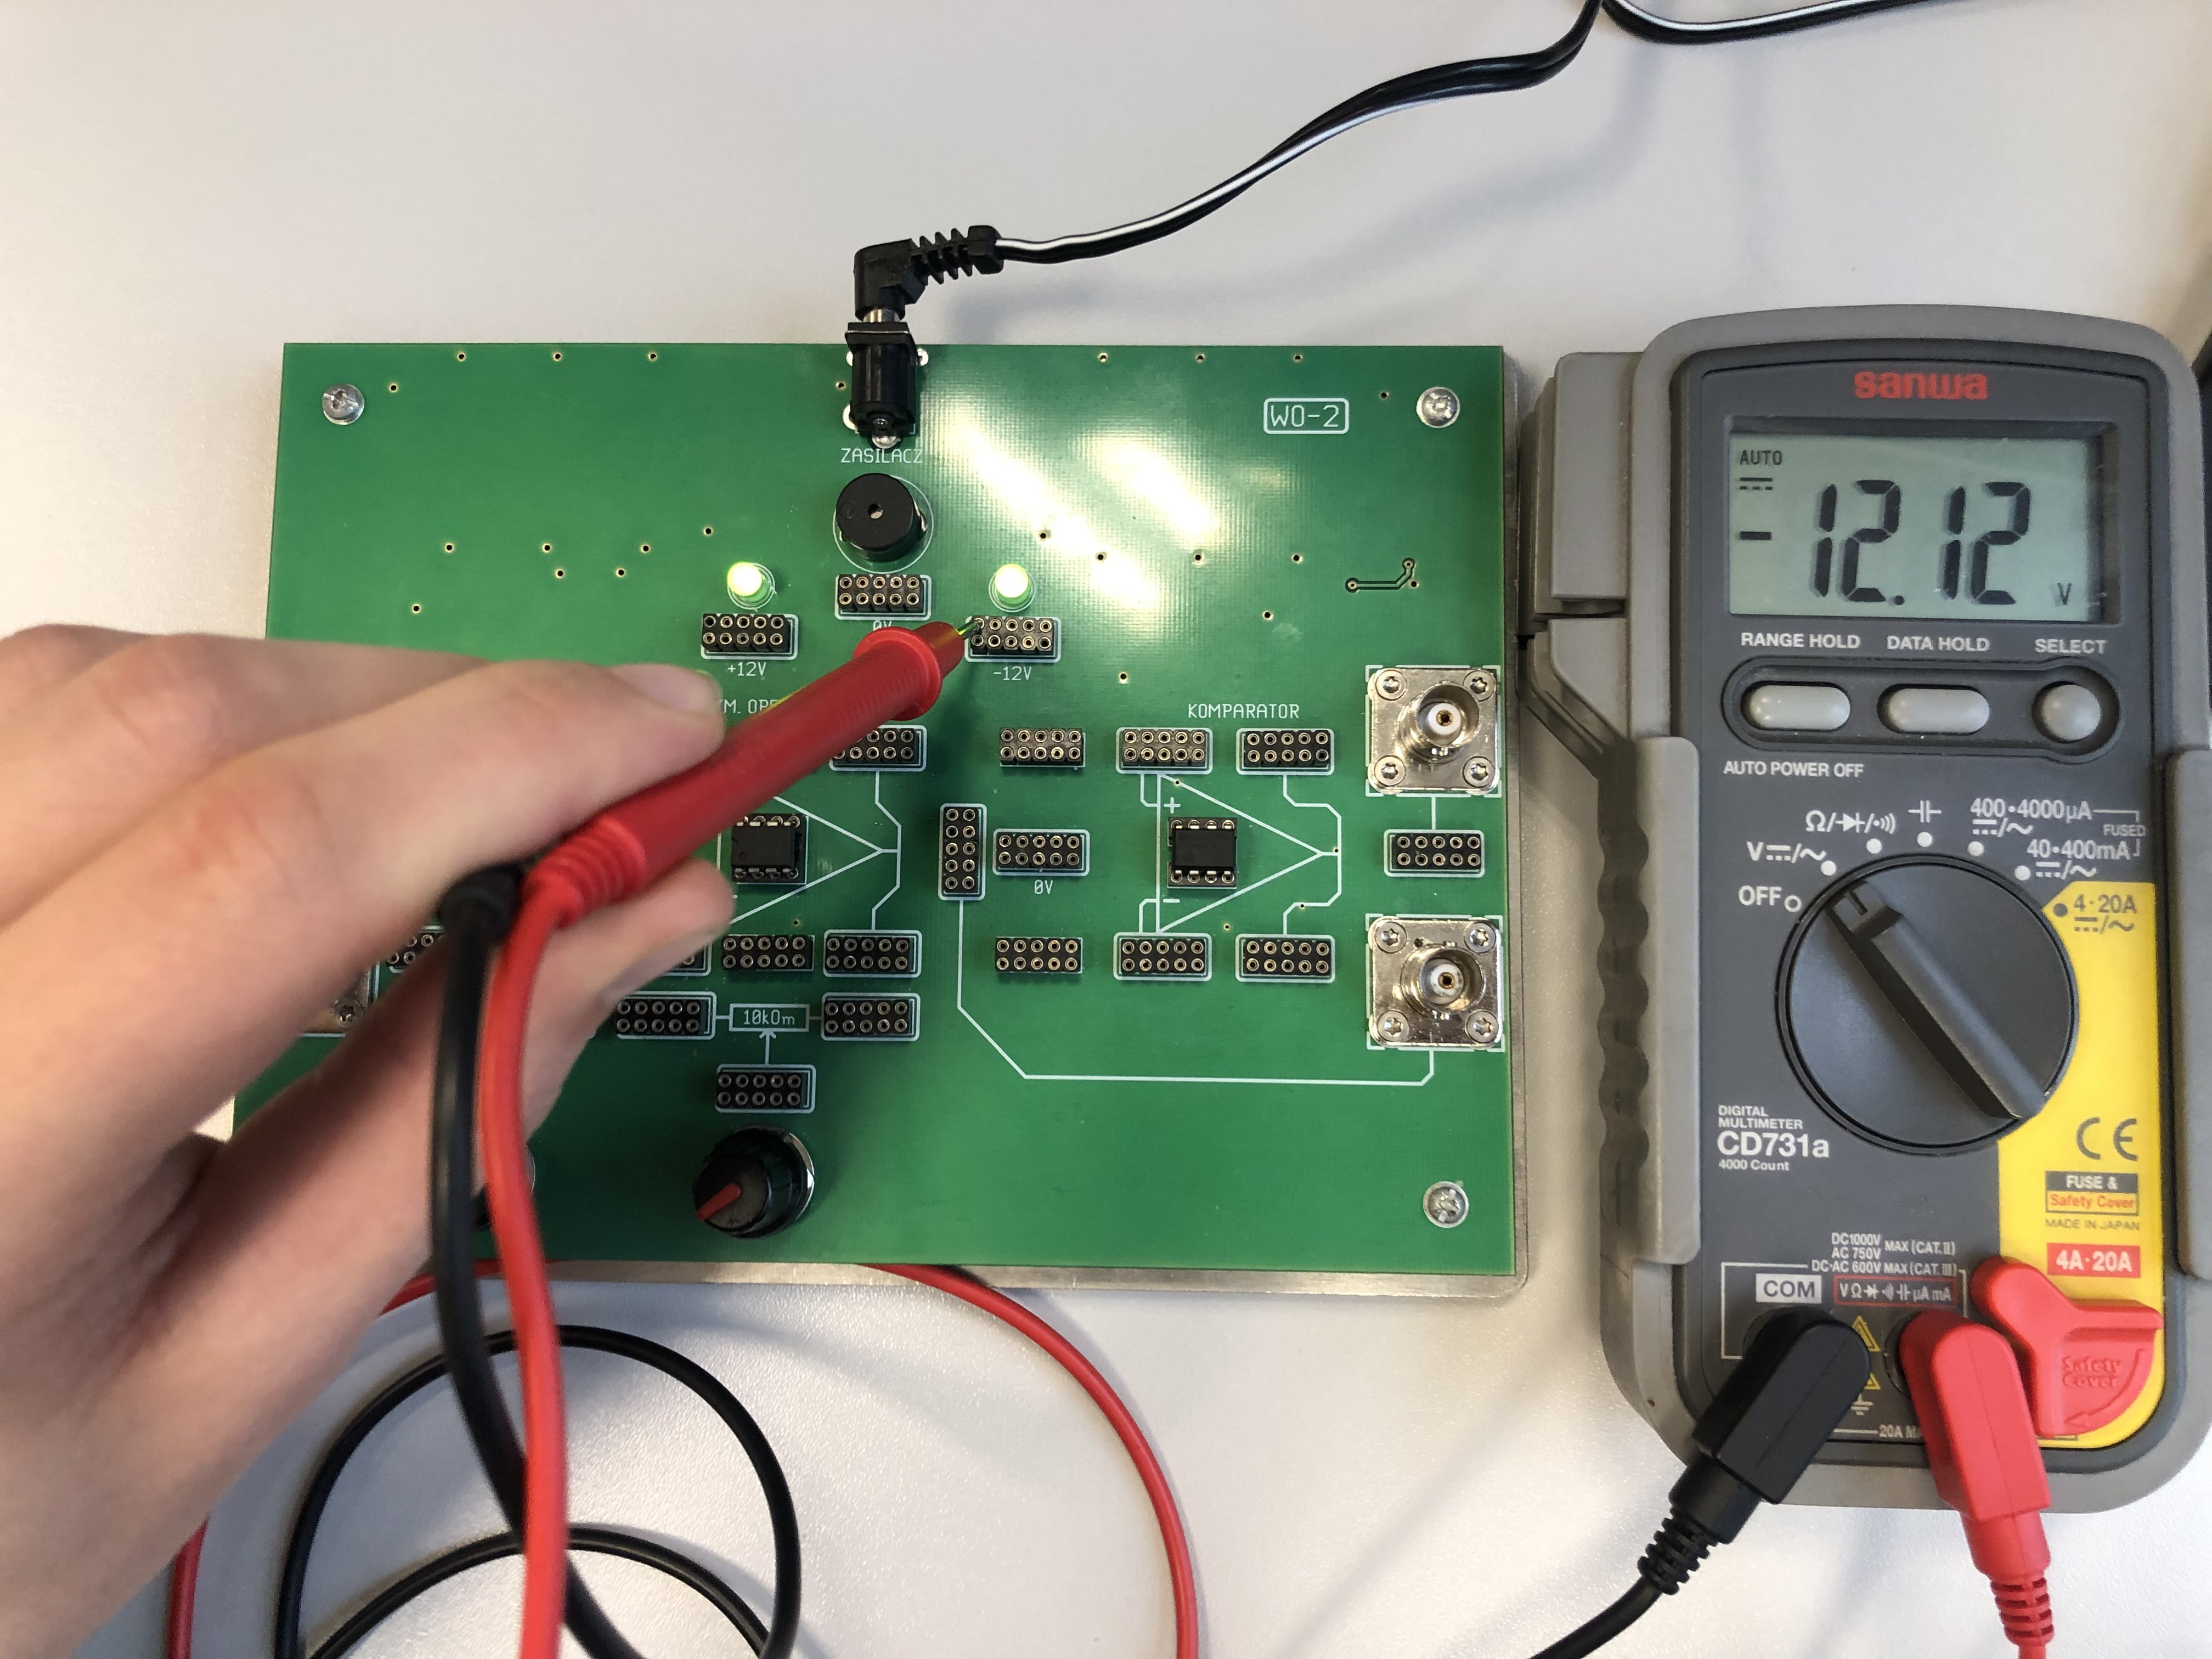
\includegraphics[width=7cm]{C9}}}%
\end{figure}

\newpage
\paragraph{Ćwiczenie 3.2 \\}
Zmontowanie wzmacniacza odwracającego fazę o wzmocnieniu 10, zdjęcie jego charakterystyki częstotliwościowej i fazowej.

\begin{figure}[H]
    \centering
    \subfloat[\centering ]{{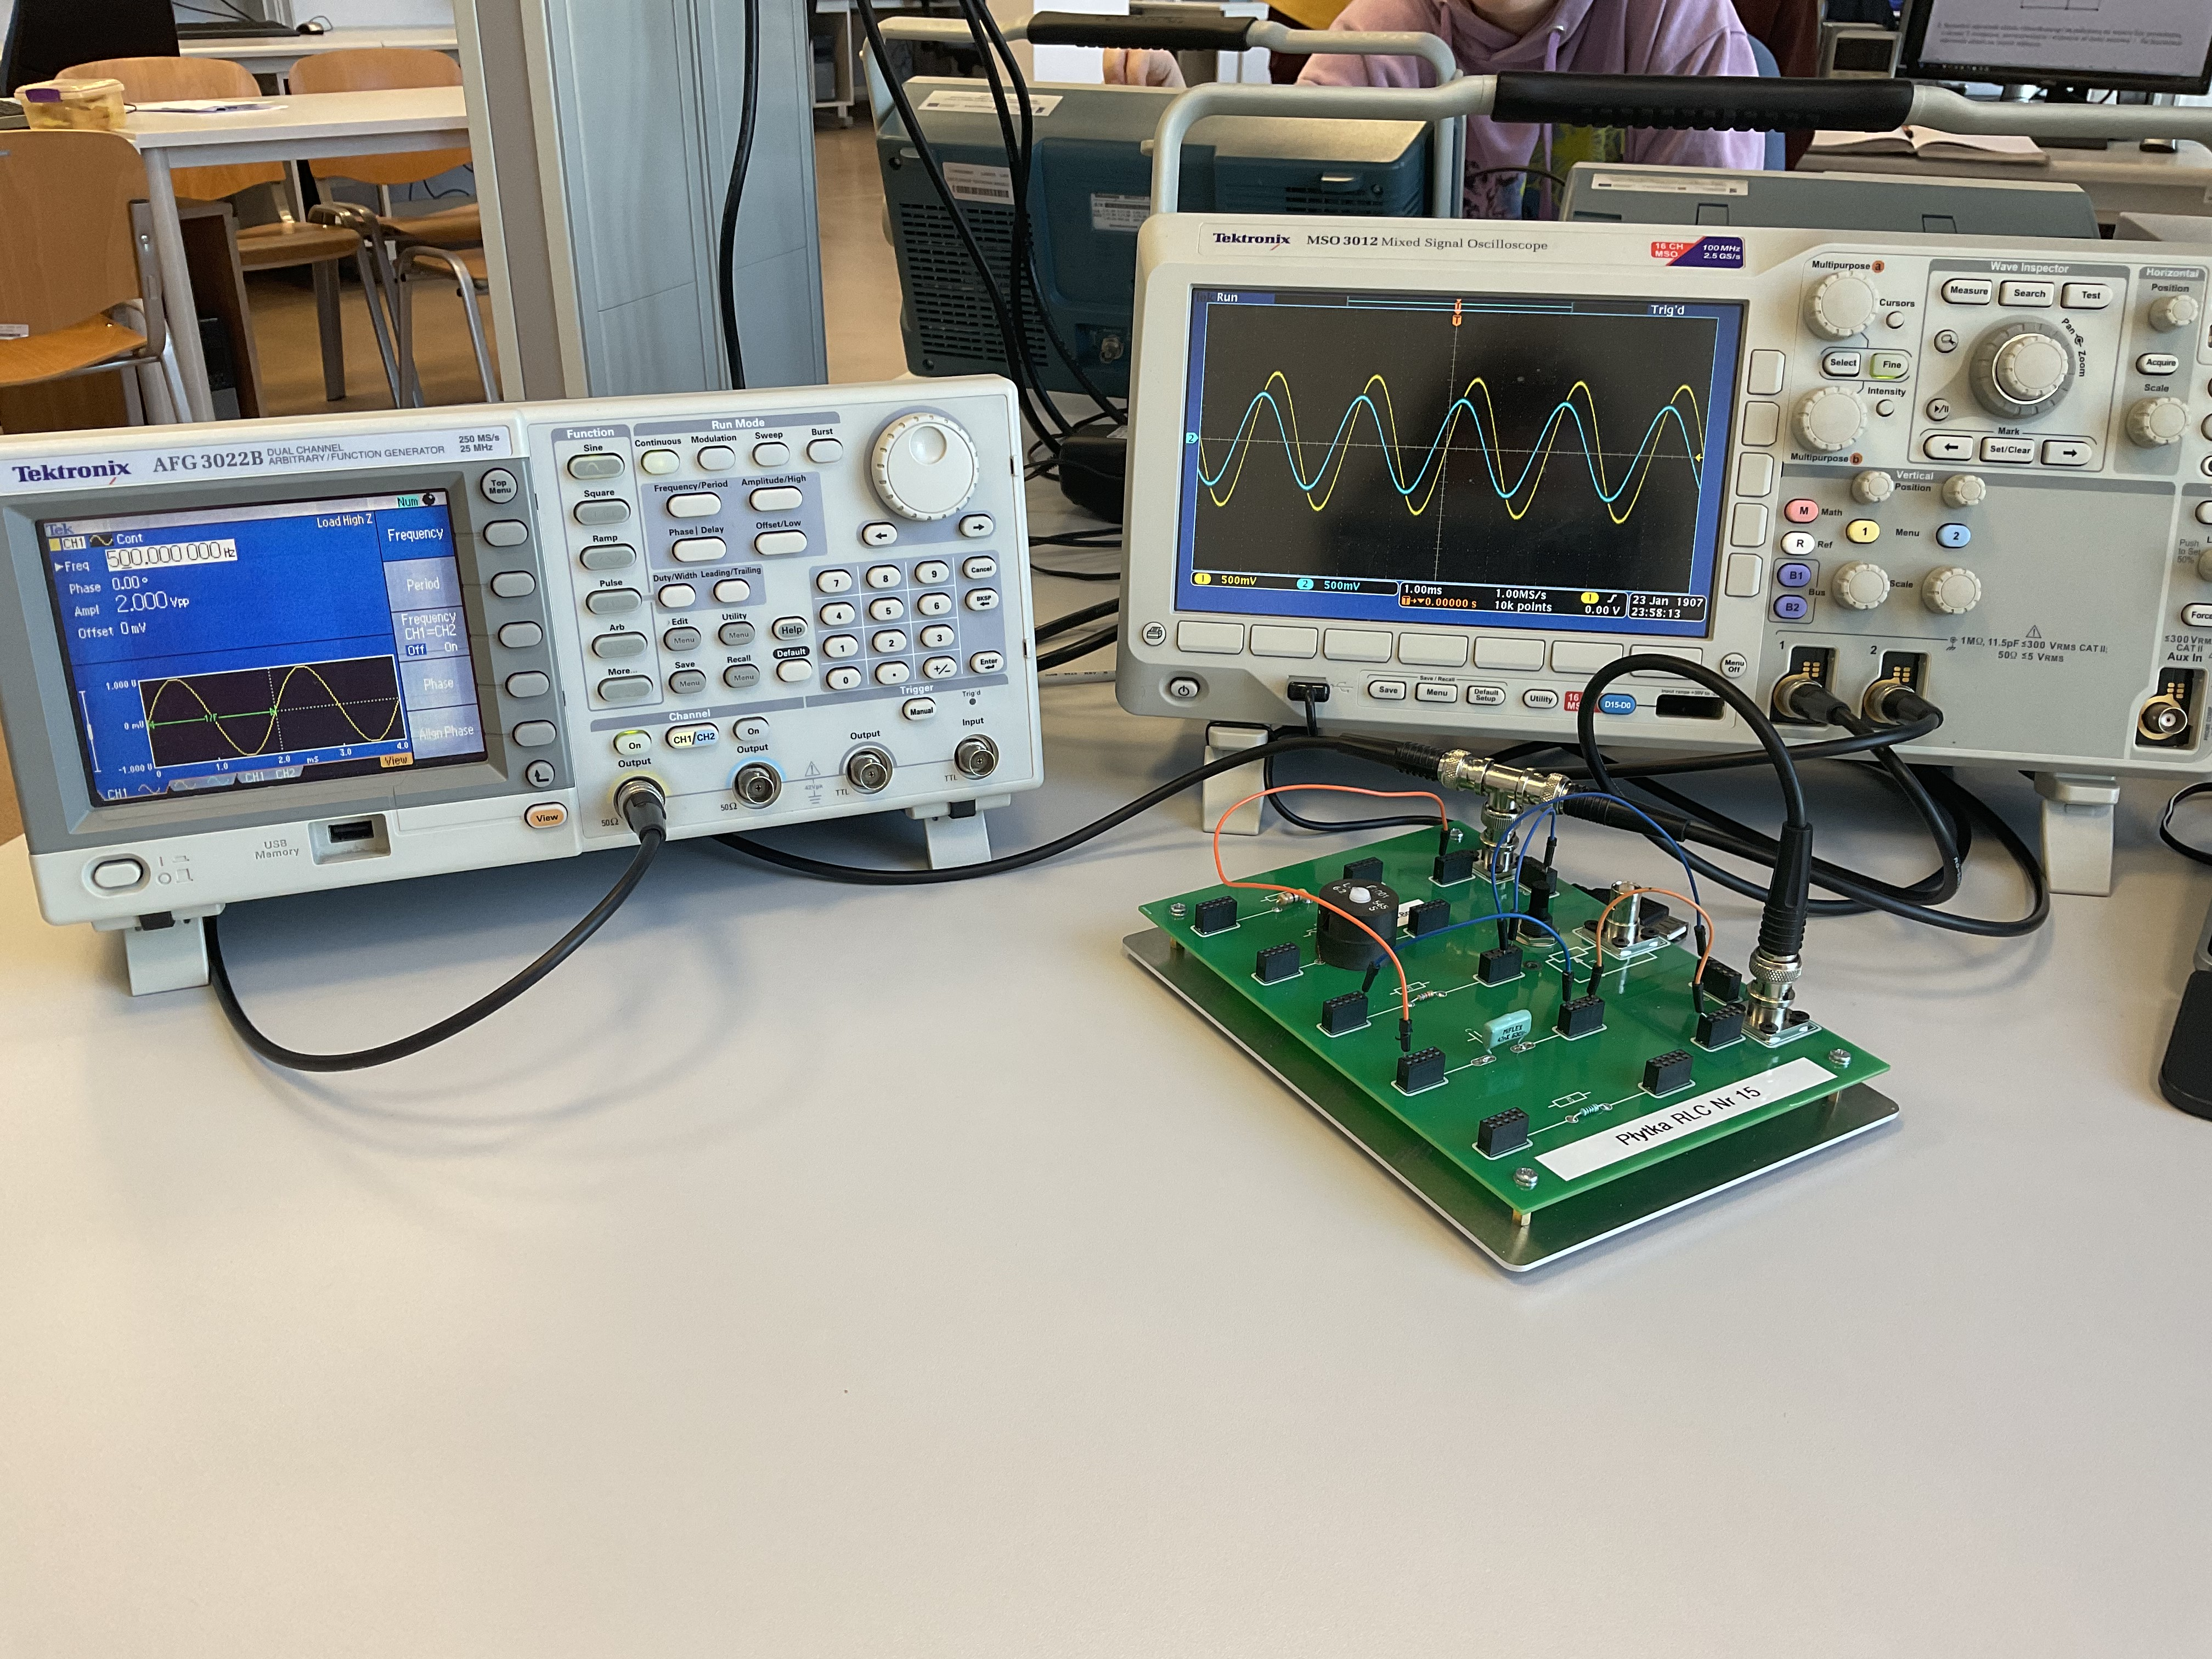
\includegraphics[width=7cm]{C1}}}%
    \qquad
    \subfloat[\centering ]{{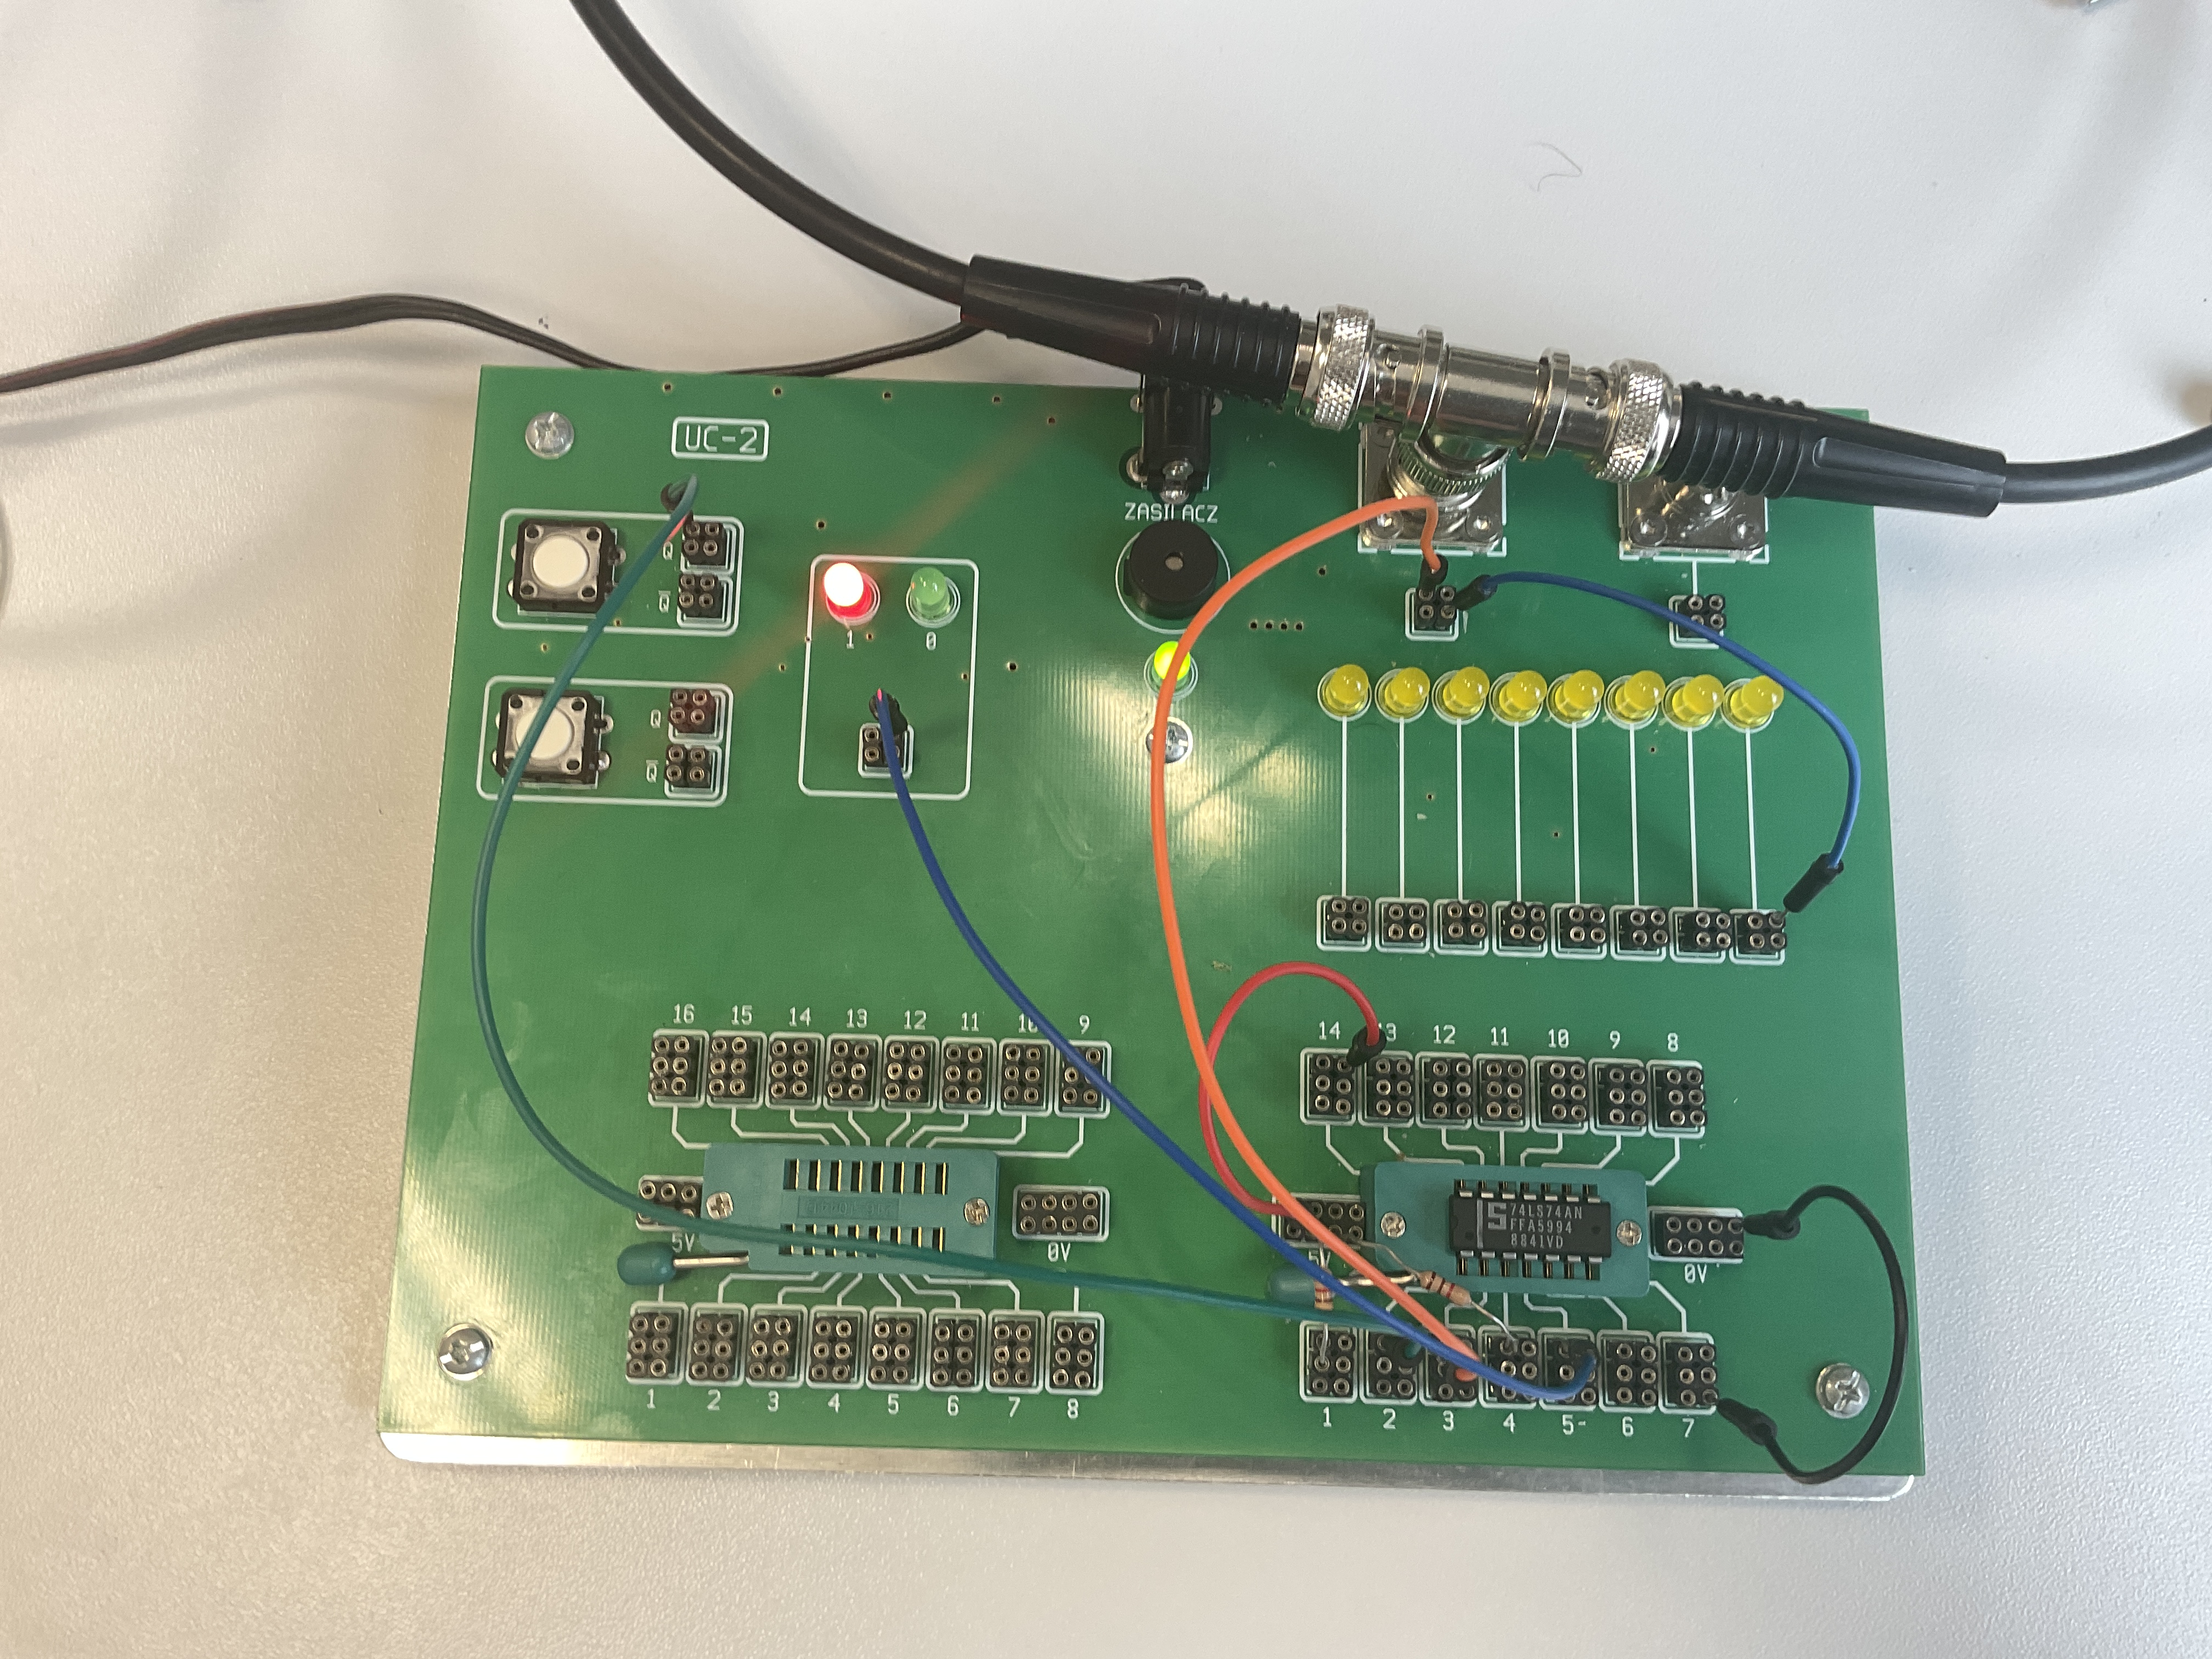
\includegraphics[width=7cm]{C2}}}%
\end{figure}

Montując ten układ użyłem rezystorów o oporze $R_f = 100 \ k \Omega$ oraz $R_1 = 10 \ k \Omega$. Wzmocnienie tego wzmacniacza powinno więc wynosić 10:

$$ U_{WY} = - \frac{R_f}{R_1} U_{WE} = - \frac{100 \ k \Omega}{10 \ k \Omega} U_{WE} = -10 U_{WE} $$

Gdzie minus przy napięciu wyjściowym oznacza odwrócenie fazy (przesu- nięcie fazy o $180^{\circ}$. \\

Podałem na wejście układu sygnał sinusoidalny o częstotliwości $1 \ kHz$ i amplitudzie $100 \ mV$pp. Napięcie na wyjściu zmierzone oscyloskopem wynosiło $1.05 \ V$pp i sygnał wyjściowy był przesunięty o około $175.8^{\circ}$ w stosunku do wejściowego.

\begin{figure}[H]
    \centering
    \subfloat[\centering Dziesięciokrotne wzmocnienie sygnału i odwrócenie fazy]{{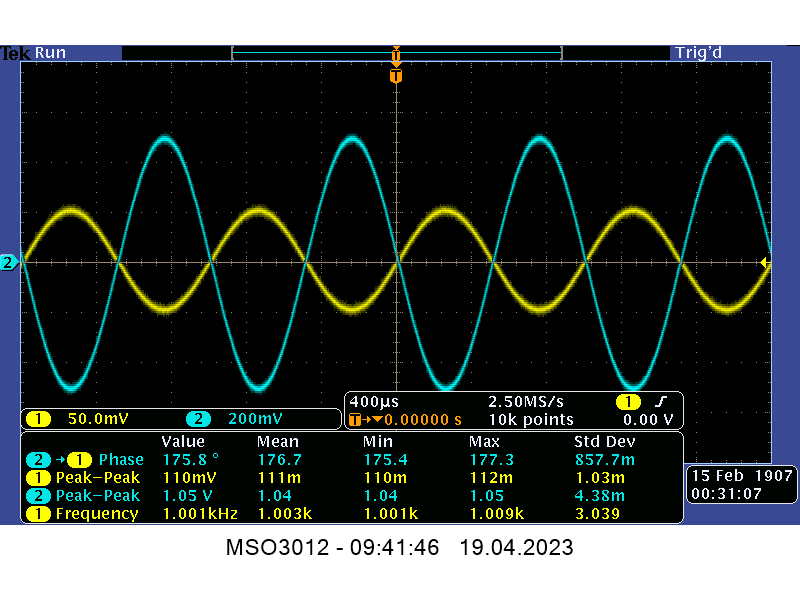
\includegraphics[width=7cm]{A0}}}%
\end{figure}

\newpage
Aby zdjąć charakterystyki amplitudową i fazową zbudowanego przeze mnie układu podałem sygnał sinusoidalny o amplitudzie $100 \ mV$pp i częstotliwości z przedziału od $100 \ Hz$ do $900 \ kHz$. Na kolejnej stronie znajdują się zrzuty ekranu z oscyloskopu (nie wszystkie pomiary, żeby nie przedłużać niepotrzebnie tego sprawozdania).

\begin{tabular}{ | m{4cm} | m{4cm}| m{4cm} | m{3.5cm} | } 
  \hline
  \textbf{Częstotliwość} & \textbf{Amplituda wyjściowa} & \textbf{Przesunięcie fazowe} & \textbf{Stosunek } $U_{WY} / U_{WE}$ \\ 
  \hline
  $100 \ Hz$ & $1.04 \ V$ & $178.5^{\circ}$ & $10.4$ \\
  \hline
  $200 \ Hz$ & $1.03 \ V$ & $176.8^{\circ}$ & $10.3$ \\
  \hline
  $300 \ Hz$ & $1.04 \ V$ & $173^{\circ}$ & $10.4$ \\
  \hline
  $400 \ Hz$ & $1.04 \ V$ & $177.7^{\circ}$ & $10.4$ \\  
  \hline
  $500 \ Hz$ & $1.05 \ V$ & $176.4^{\circ}$ & $10.5$ \\
  \hline
  $600 \ Hz$ & $1.03 \ V$ & $177^{\circ}$ & $10.3$ \\
  \hline
  $700 \ Hz$ & $1.04 \ V$ & $176.9^{\circ}$ & $10.4$ \\
  \hline
  $800 \ Hz$ & $1.05 \ V$ & $175.7^{\circ}$ & $10.5$ \\
  \hline
  $900 \ Hz$ & $1.03 \ V$ & $175^{\circ}$ & $10.3$ \\
  \hline
  $1 \ kHz$ & $1.03 \ V$ & $176^{\circ}$ & $10.3$ \\
  \hline
  $2 \ kHz$ & $1.04 \ V$ & $175.5^{\circ}$ & $10.4$ \\
  \hline
  $3 \ kHz$ & $1.03 \ V$ & $176.1^{\circ}$ & $10.3$ \\
  \hline
  $4 \ kHz$ & $1.04 \ V$ & $173.1^{\circ}$ & $10.4$ \\
  \hline
  $5 \ kHz$ & $1.04 \ V$ & $173^{\circ}$ & $10.4$ \\
  \hline
  $6 \ kHz$ & $1.03 \ V$ & $175.2^{\circ}$ & $10.3$ \\
  \hline
  $7 \ kHz$ & $1.03 \ V$ & $173.7^{\circ}$ & $10.3$ \\
  \hline
  $8 \ kHz$ & $1.04 \ V$ & $172.9^{\circ}$ & $10.4$ \\
  \hline
  $9 \ kHz$ & $1.03 \ V$ & $172.1^{\circ}$ & $10.3$ \\
  \hline
  $10 \ kHz$ & $1.04 \ V$ & $173.2^{\circ}$ & $10.4$ \\
  \hline
  $20 \ kHz$ & $1.02 \ V$ & $163.9^{\circ}$ & $10.2$ \\
  \hline
  $30 \ kHz$ & $1 \ V$ & $156^{\circ}$ & $10$ \\
  \hline
  $40 \ kHz$ & $960 \ mV$ & $148.8^{\circ}$ & $9.6$ \\
  \hline
  $50 \ kHz$ & $928 \ mV$ & $144.1^{\circ}$ & $9.28$ \\
  \hline
  $60 \ kHz$ & $880 \ mV$ & $139^{\circ}$ & $8.8$ \\
  \hline
  $70 \ kHz$ & $832 \ mV$ & $132^{\circ}$ & $8.32$ \\
  \hline
  $80 \ kHz$ & $792 \ mV$ & $130.4^{\circ}$ & $7.92$ \\
  \hline
  $90 \ kHz$ & $752 \ mV$ & $127.7^{\circ}$ & $7.52$ \\
  \hline
  $100 \ kHz$ & $712 \ mV$ & $121.7^{\circ}$ & $7.12$ \\
  \hline
  $200 \ kHz$ & $440 \ mV$ & $97.69^{\circ}$ & $4.4$ \\
  \hline
  $300 \ kHz$ & $286 \ mV$ & $88.38^{\circ}$ & $2.86$ \\
  \hline
  $400 \ kHz$ & $216 \ mV$ & $79.96^{\circ}$ & $2.16$ \\
  \hline
  $500 \ kHz$ & $174 \ mV$ & $70.81^{\circ}$ & $1.74$ \\
  \hline
  $600 \ kHz$ & $138 \ mV$ & $65.04^{\circ}$ & $1.38$ \\
  \hline
  $700 \ kHz$ & $117 \ mV$ & $58.04^{\circ}$ & $1.17$ \\
  \hline
  $800 \ kHz$ & $102 \ mV$ & $51.72^{\circ}$ & $1.02$ \\
  \hline
  $900 \ kHz$ & $88 \ mV$ & $47.91^{\circ}$ & $0.88$ \\
  \hline
\end{tabular}

\newpage

\begin{figure}[H]
    \centering
    \subfloat[\centering $100 \ Hz$]{{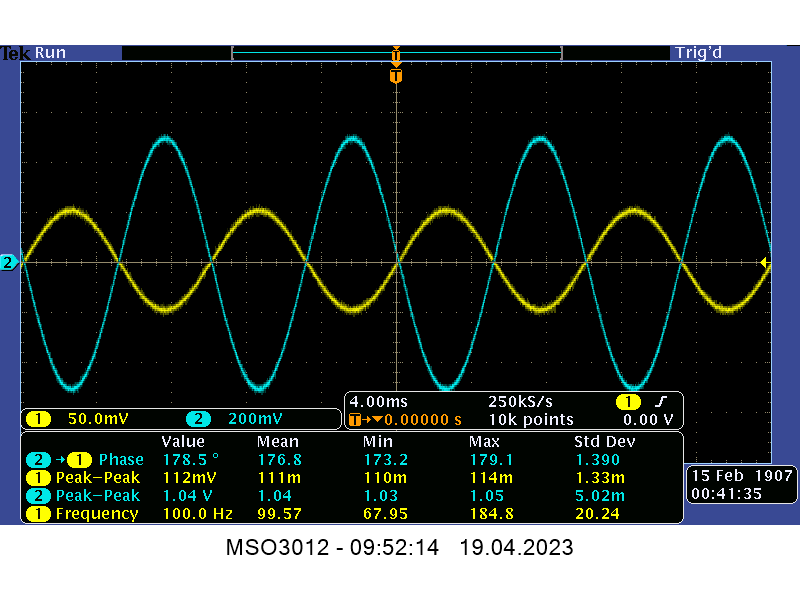
\includegraphics[width=7cm]{A1}}}%
    \qquad
    \subfloat[\centering $300 \ Hz$]{{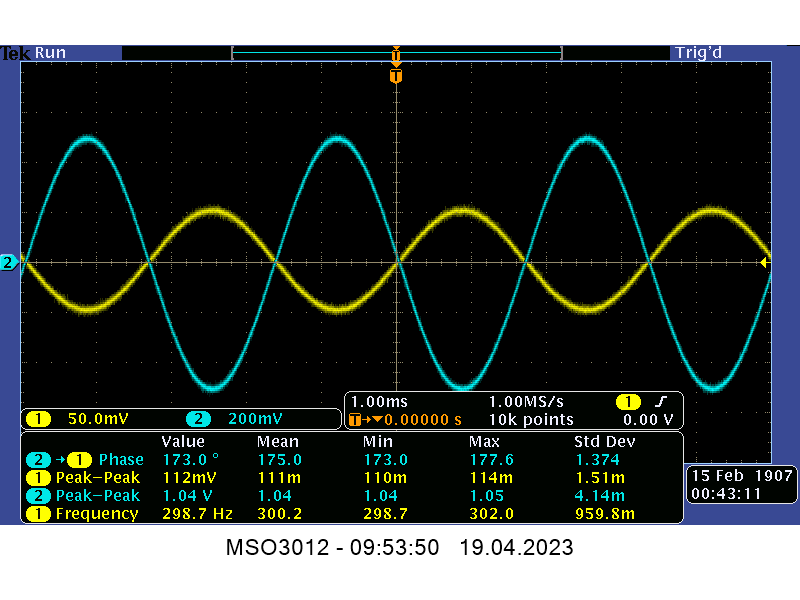
\includegraphics[width=7cm]{A3}}}%
\end{figure}

\begin{figure}[H]
    \centering
    \subfloat[\centering $400 \ Hz$]{{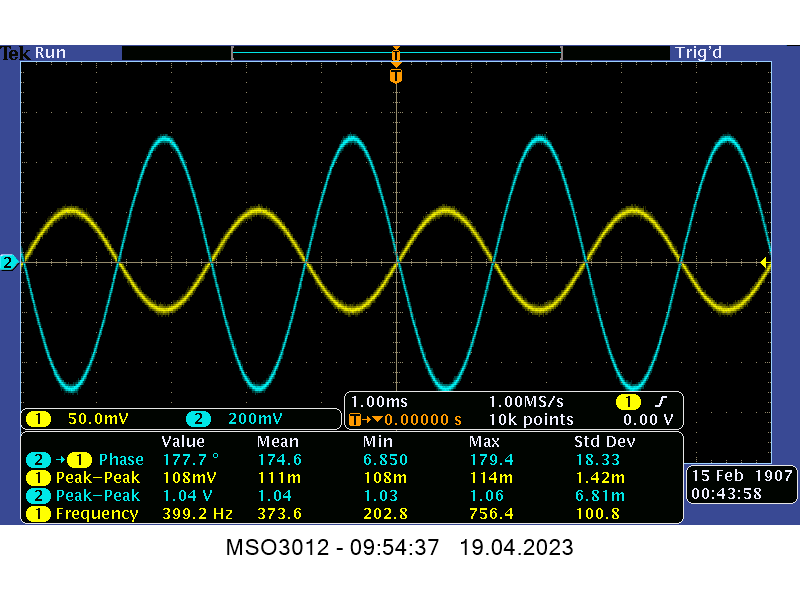
\includegraphics[width=7cm]{A4}}}%
    \qquad
    \subfloat[\centering $500 \ Hz$]{{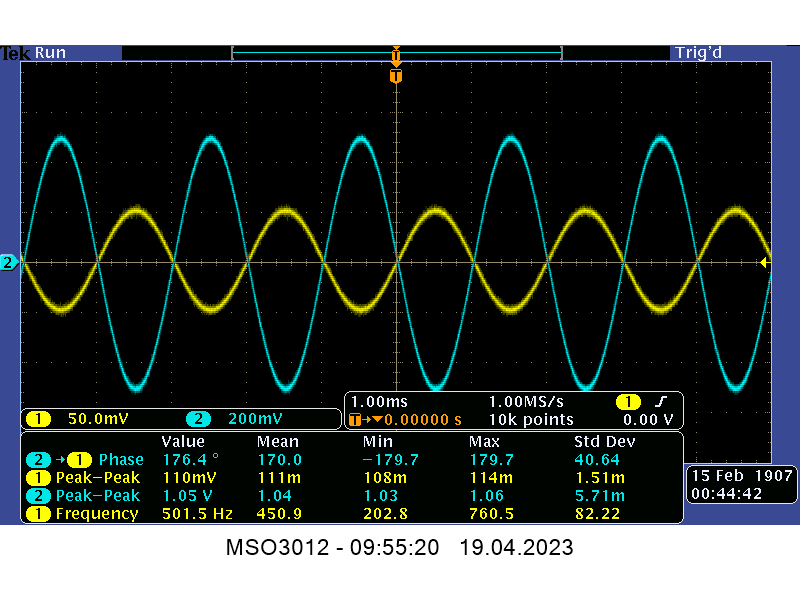
\includegraphics[width=7cm]{A5}}}%
\end{figure}

\begin{figure}[H]
    \centering
    \subfloat[\centering $600 \ Hz$]{{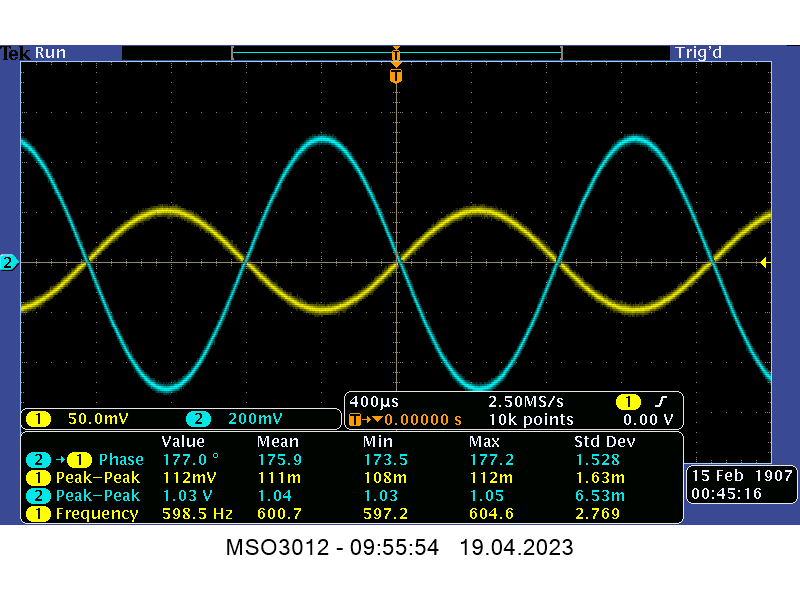
\includegraphics[width=7cm]{A6}}}%
    \qquad
    \subfloat[\centering $1 \ kHz$]{{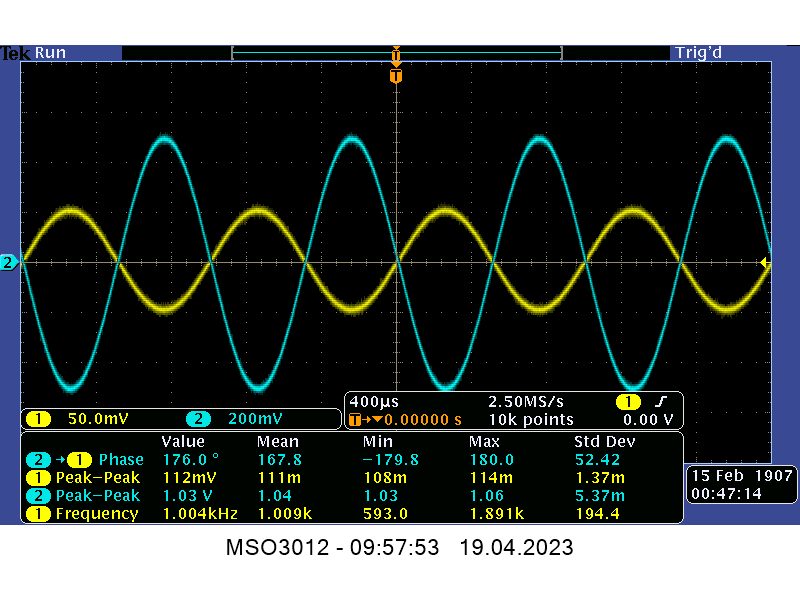
\includegraphics[width=7cm]{A7}}}%
\end{figure}

\begin{figure}[H]
    \centering
    \subfloat[\centering $5 \ kHz$]{{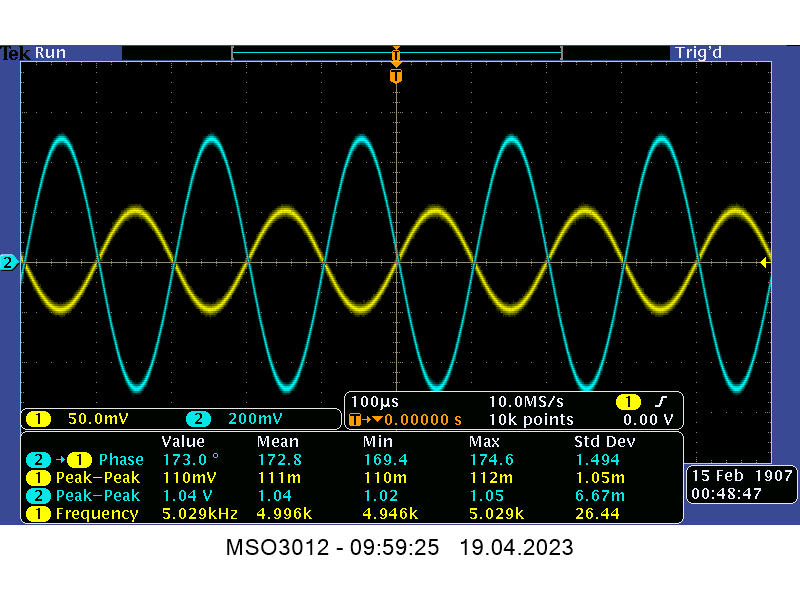
\includegraphics[width=7cm]{A8}}}%
    \qquad
    \subfloat[\centering $10 \ kHz$]{{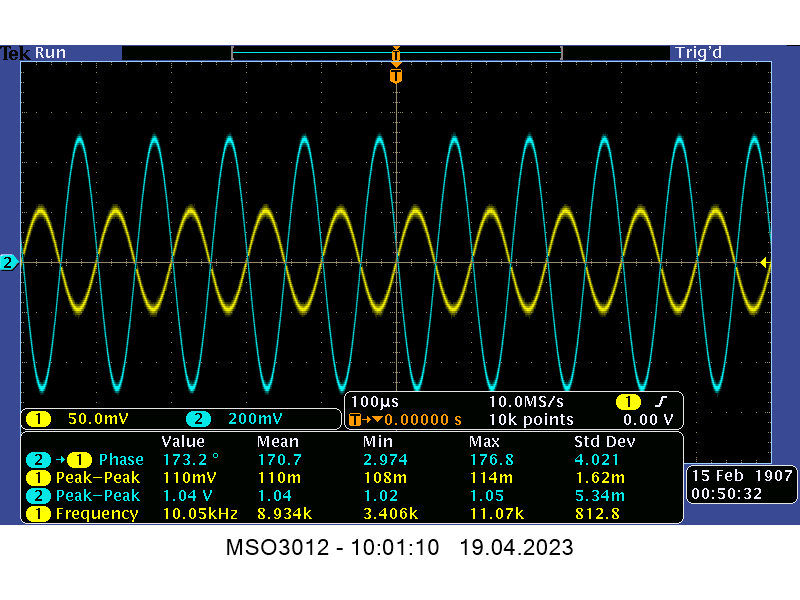
\includegraphics[width=7cm]{A9}}}%
\end{figure}

\begin{figure}[H]
    \centering
    \subfloat[\centering $20 \ kHz$]{{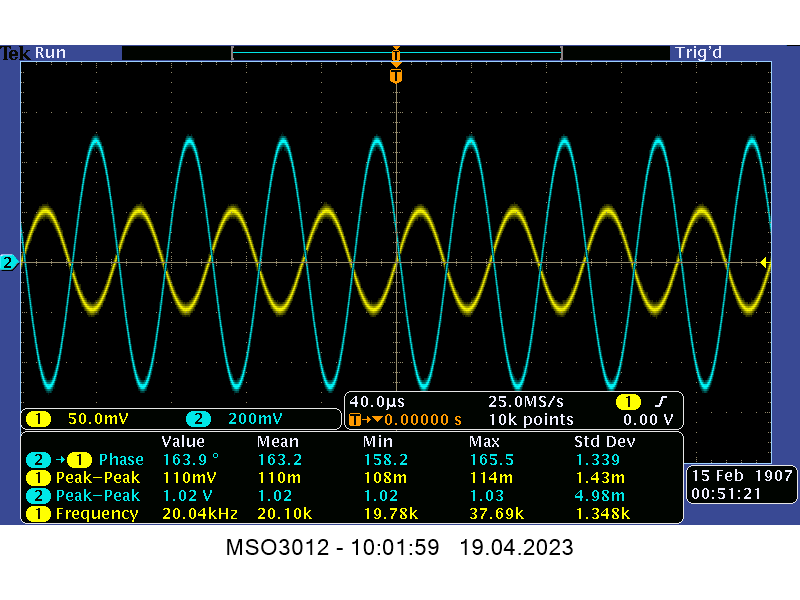
\includegraphics[width=7cm]{A10}}}%
    \qquad
    \subfloat[\centering $30 \ kHz$]{{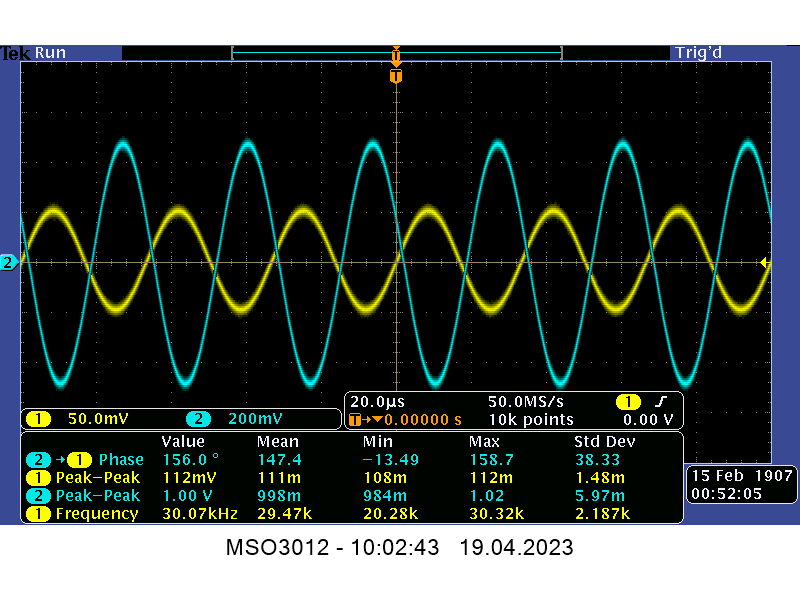
\includegraphics[width=7cm]{A11}}}%
\end{figure}

\begin{figure}[H]
    \centering
    \subfloat[\centering $100 \ kHz$]{{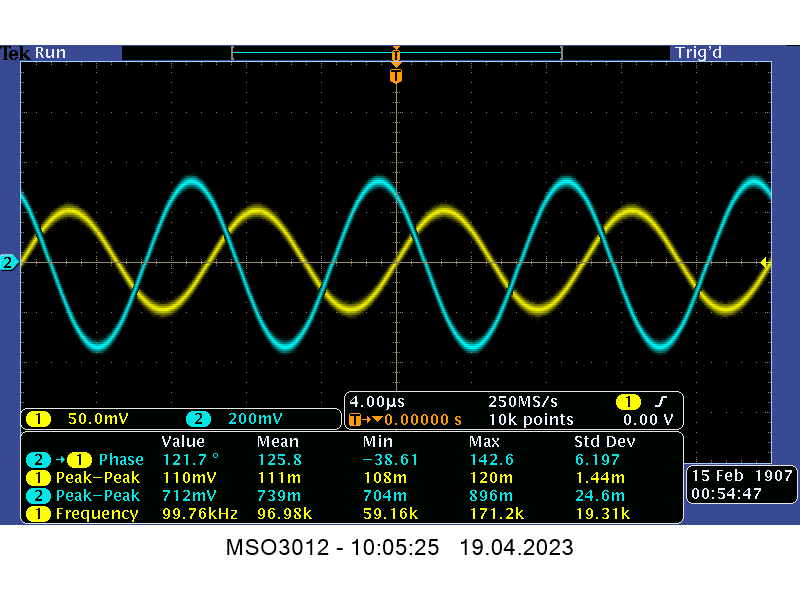
\includegraphics[width=7cm]{A12}}}%
    \qquad
    \subfloat[\centering $200 \ kHz$]{{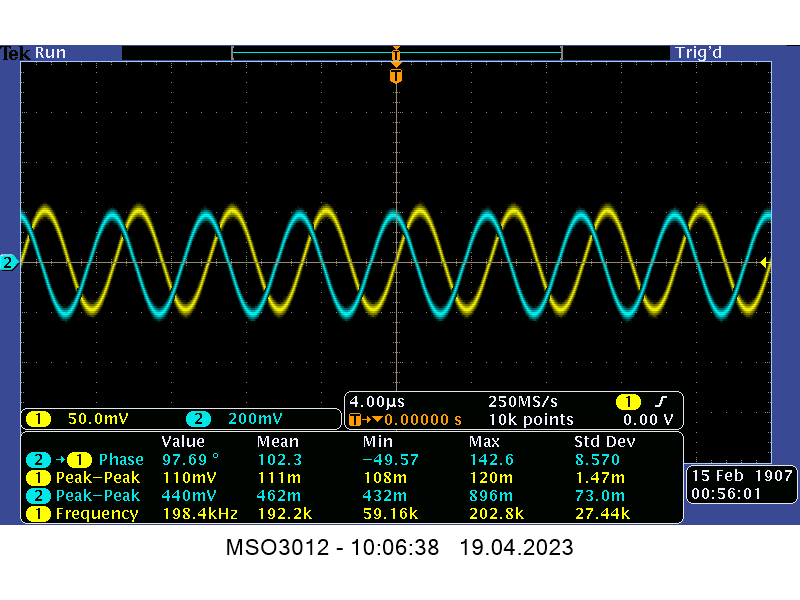
\includegraphics[width=7cm]{A13}}}%
\end{figure}

\begin{figure}[H]
    \centering
    \subfloat[\centering $300 \ kHz$]{{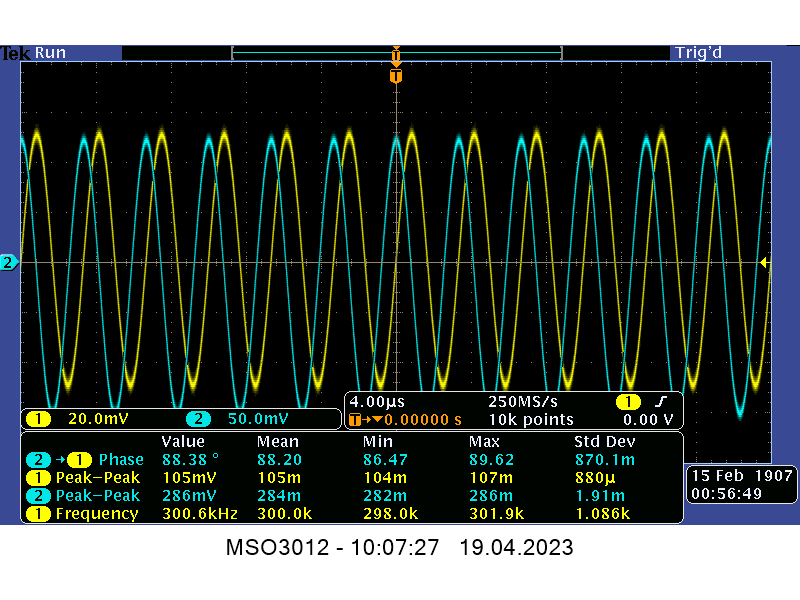
\includegraphics[width=7cm]{A14}}}%
    \qquad
    \subfloat[\centering $700 \ kHz$]{{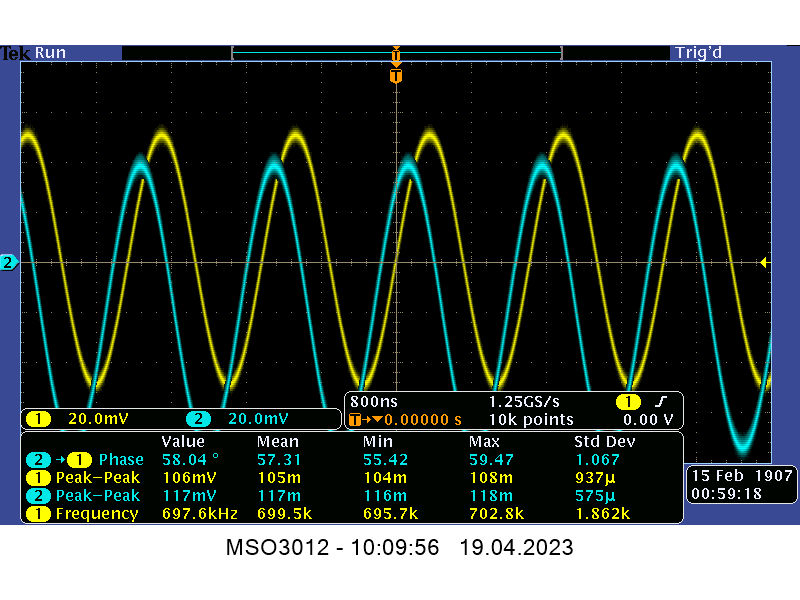
\includegraphics[width=7cm]{A15}}}%
\end{figure}

\begin{figure}[H]
    \centering
    \subfloat[\centering $800 \ kHz$]{{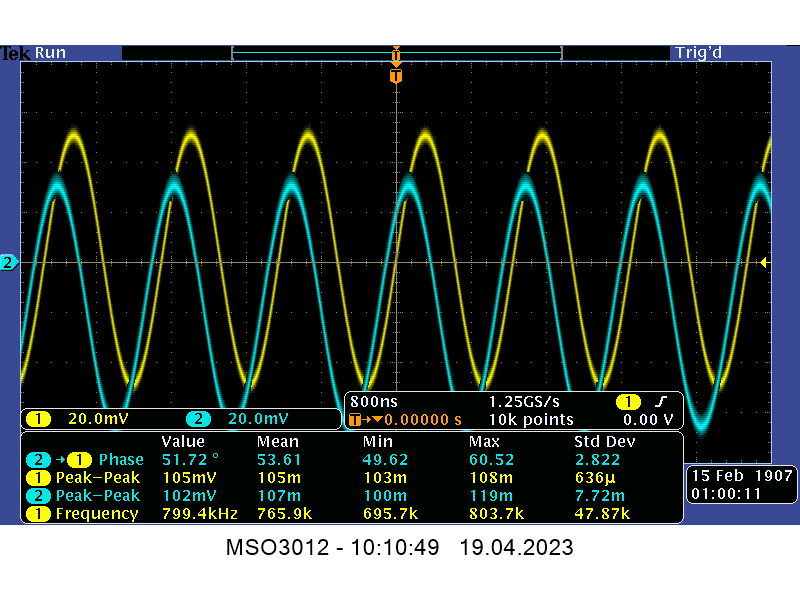
\includegraphics[width=7cm]{A16}}}%
    \qquad
    \subfloat[\centering $900 \ kHz$]{{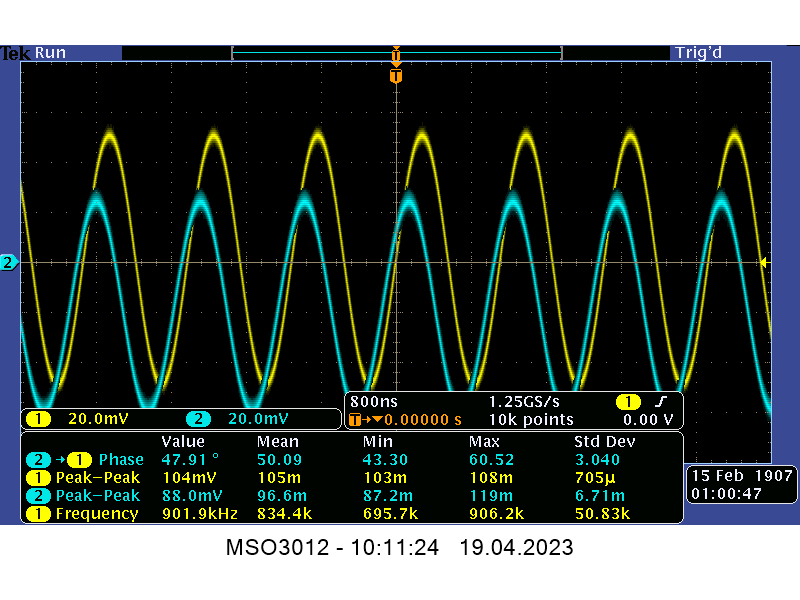
\includegraphics[width=7cm]{A17}}}%
\end{figure}



\newpage
\paragraph{Notatki z zeszytu labolatoryjnego \\}
Poniżej załączone są notatki z zeszytu labolatoryjnego, które prowadziłem podczas zajęć wykonując pomiary.

\begin{figure}[H]
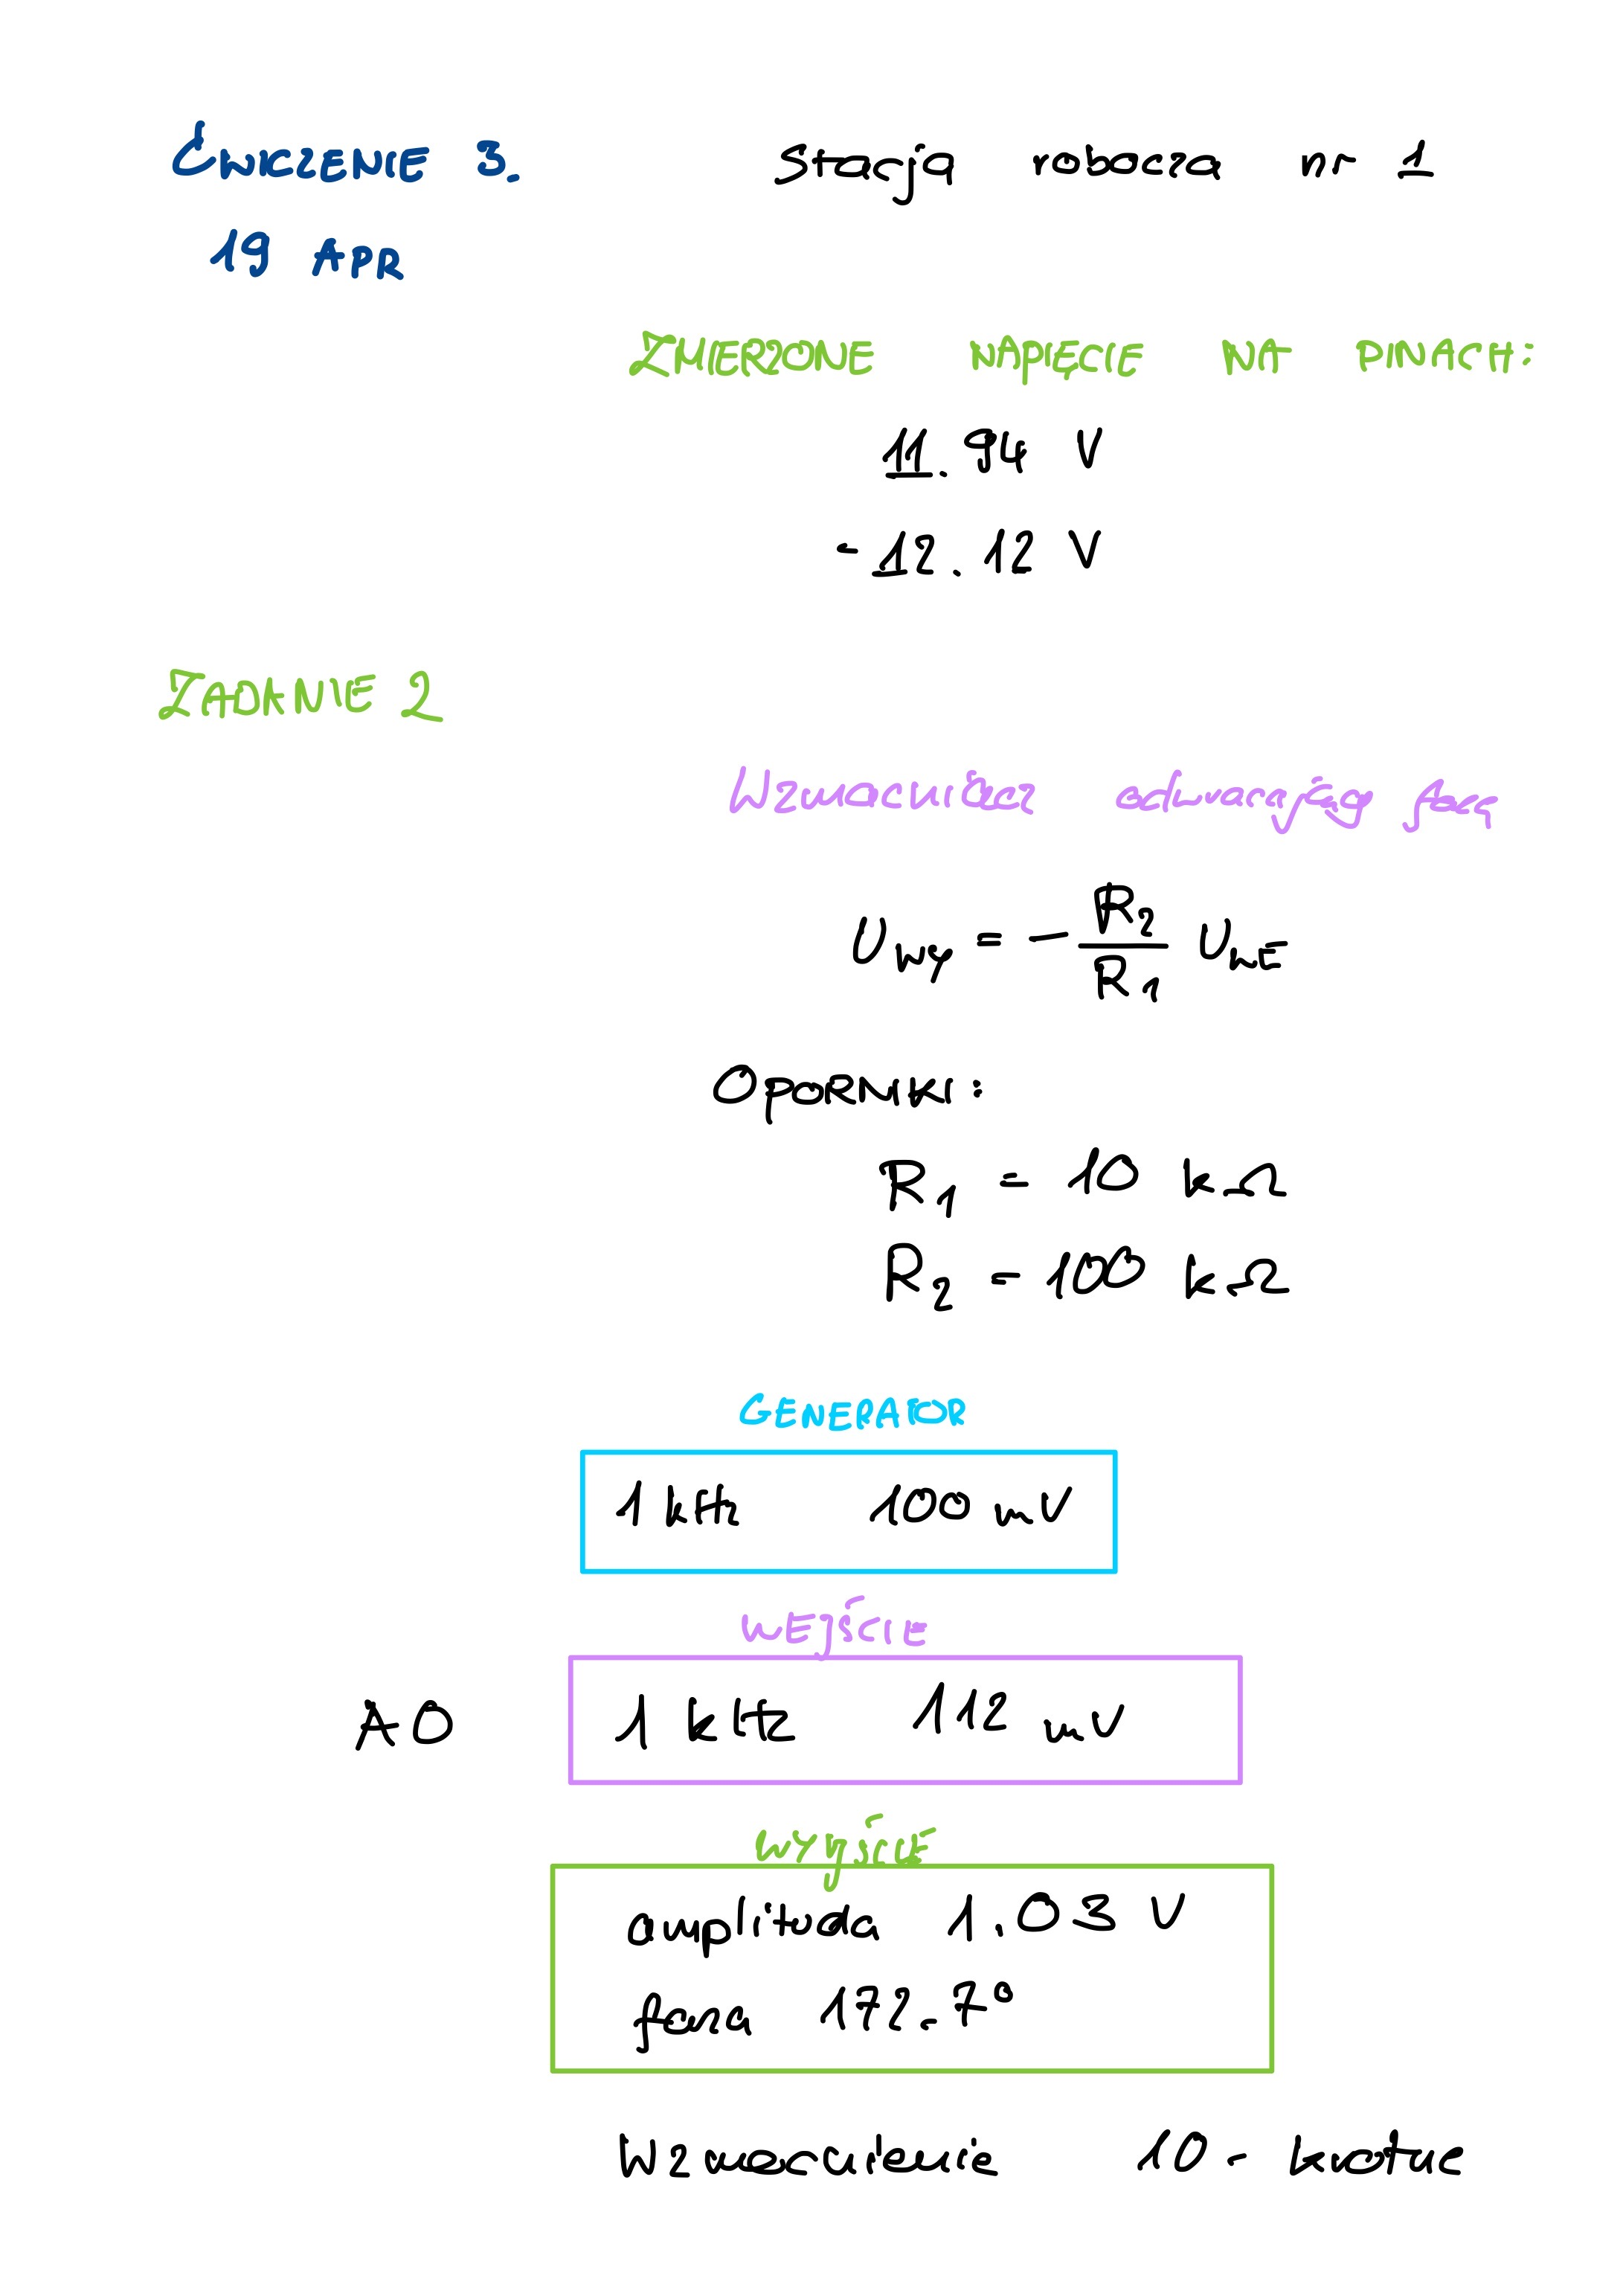
\includegraphics[scale=0.2]{B0}
\centering
\captionsetup{labelformat=empty}
\caption{}
\end{figure}

\begin{figure}[H]
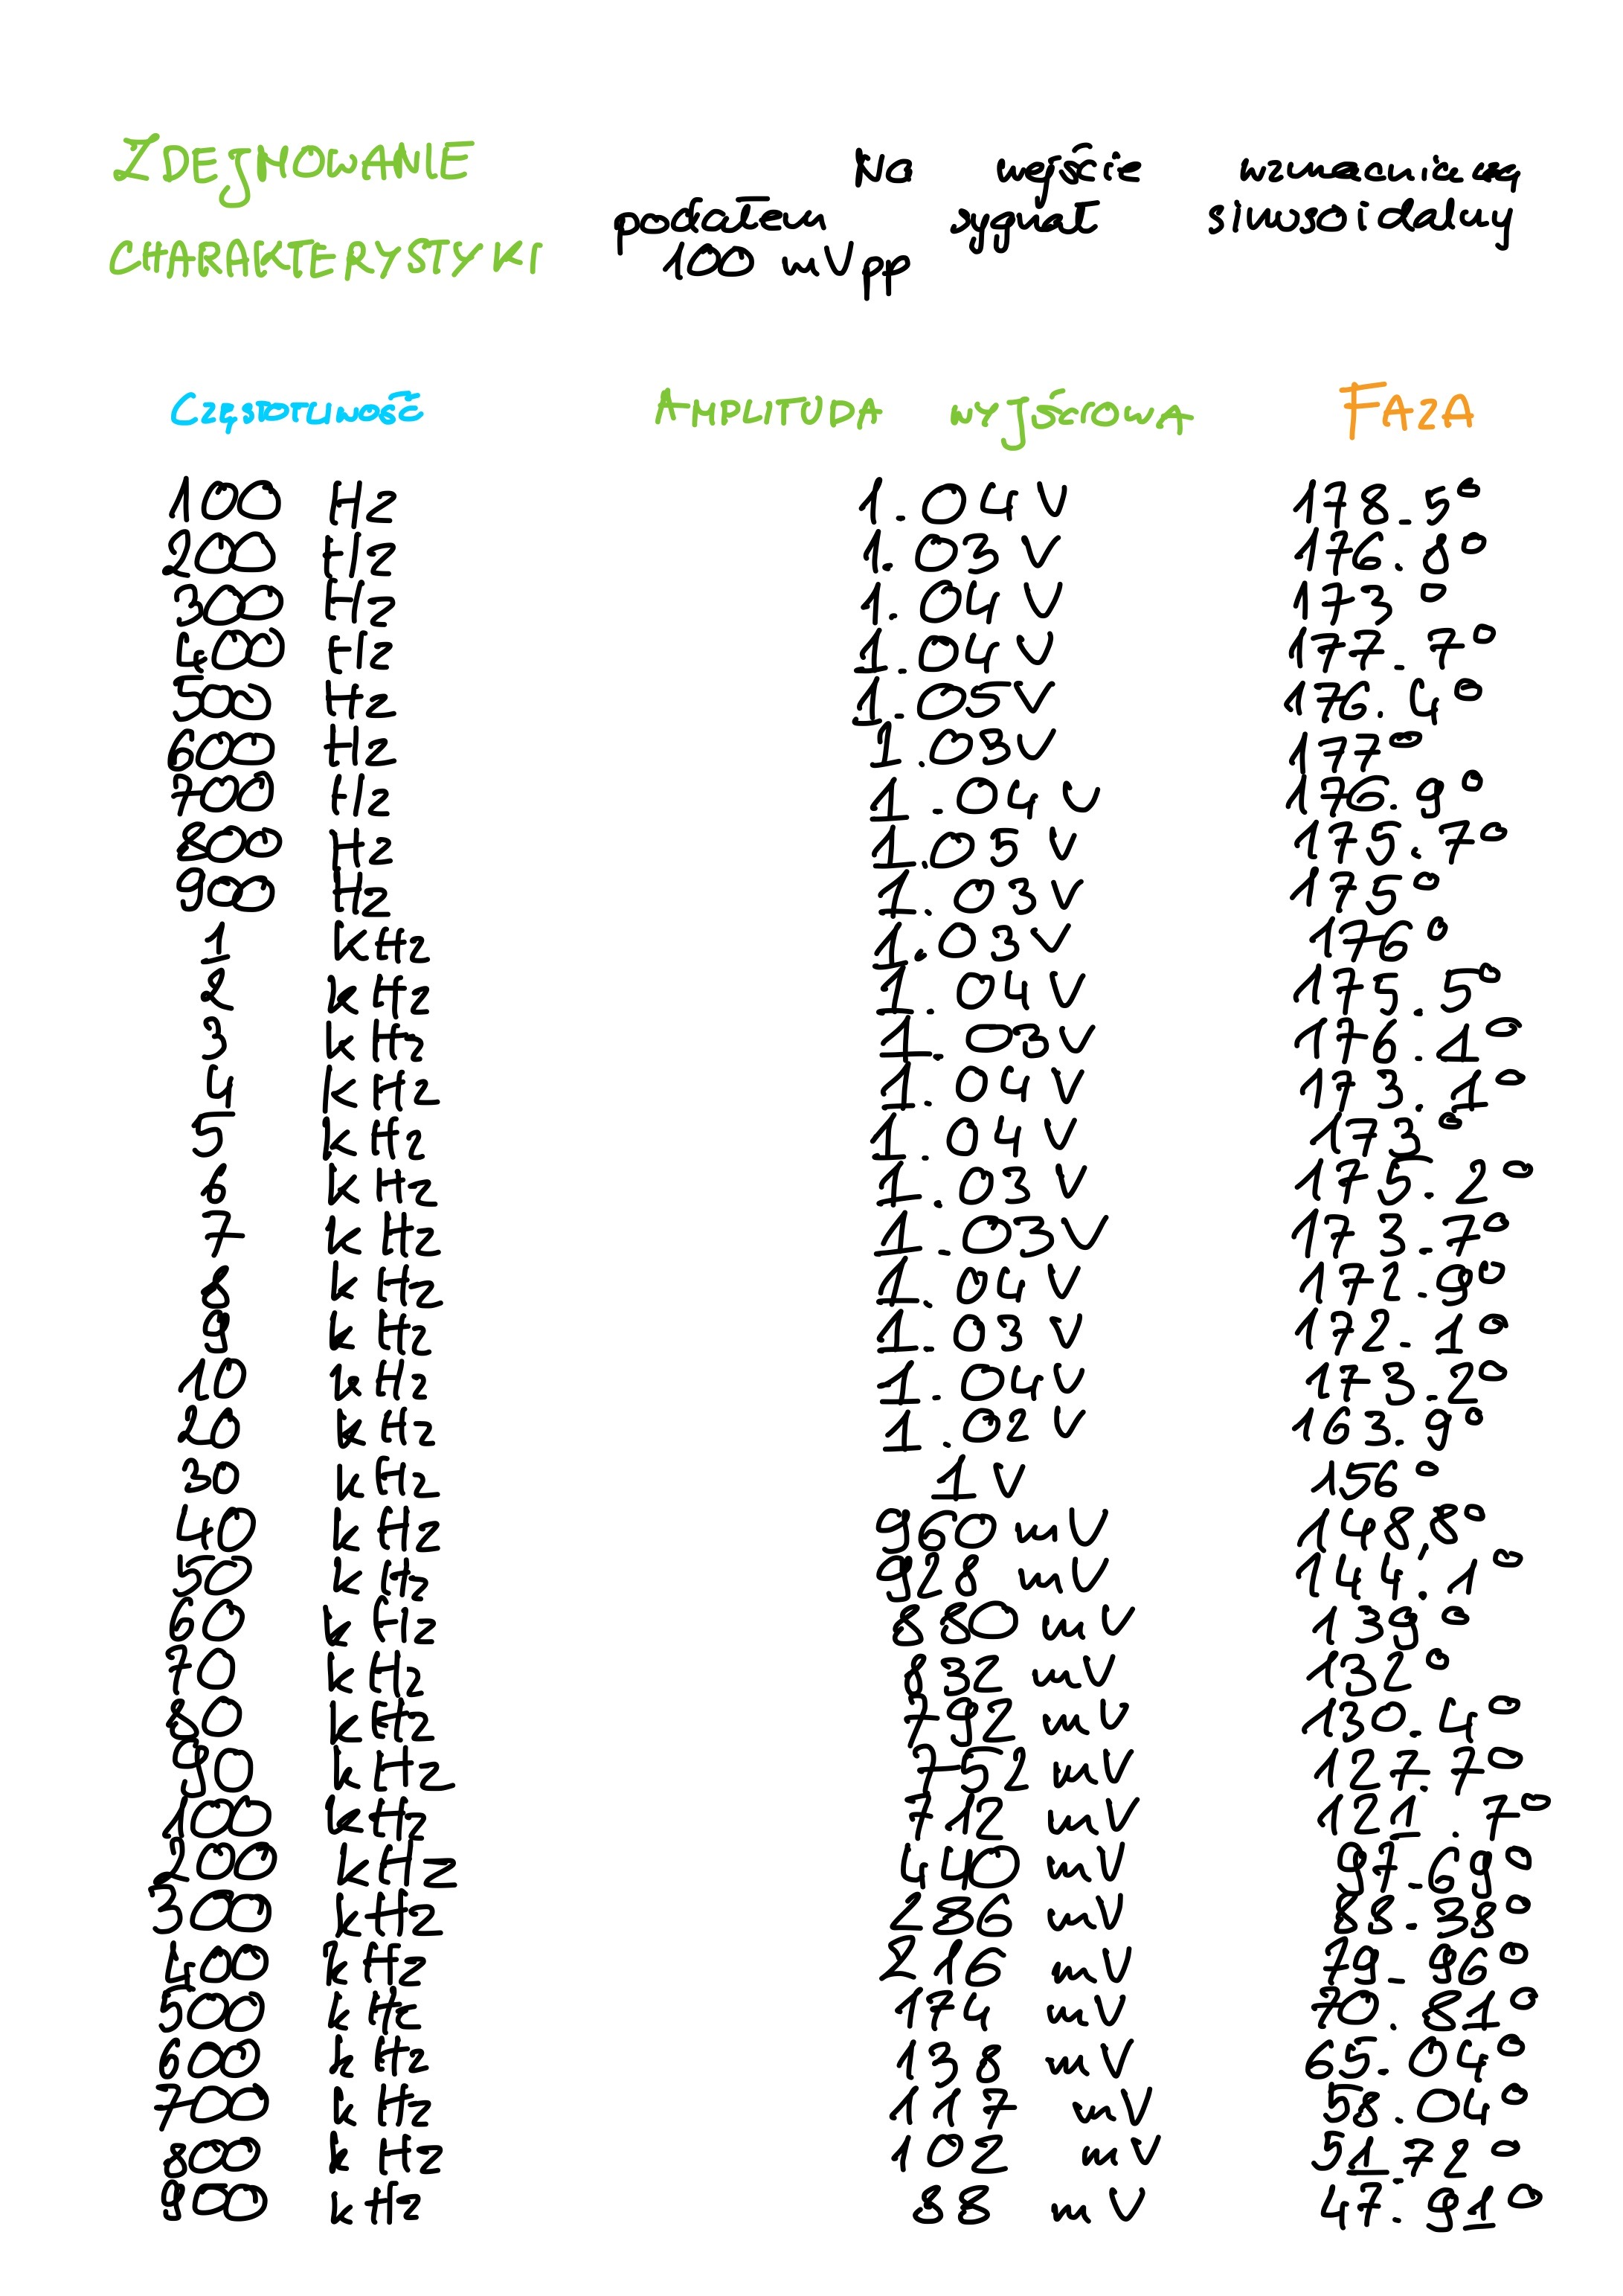
\includegraphics[scale=0.2]{B1}
\centering
\captionsetup{labelformat=empty}
\caption{}
\end{figure}

\begin{figure}[H]
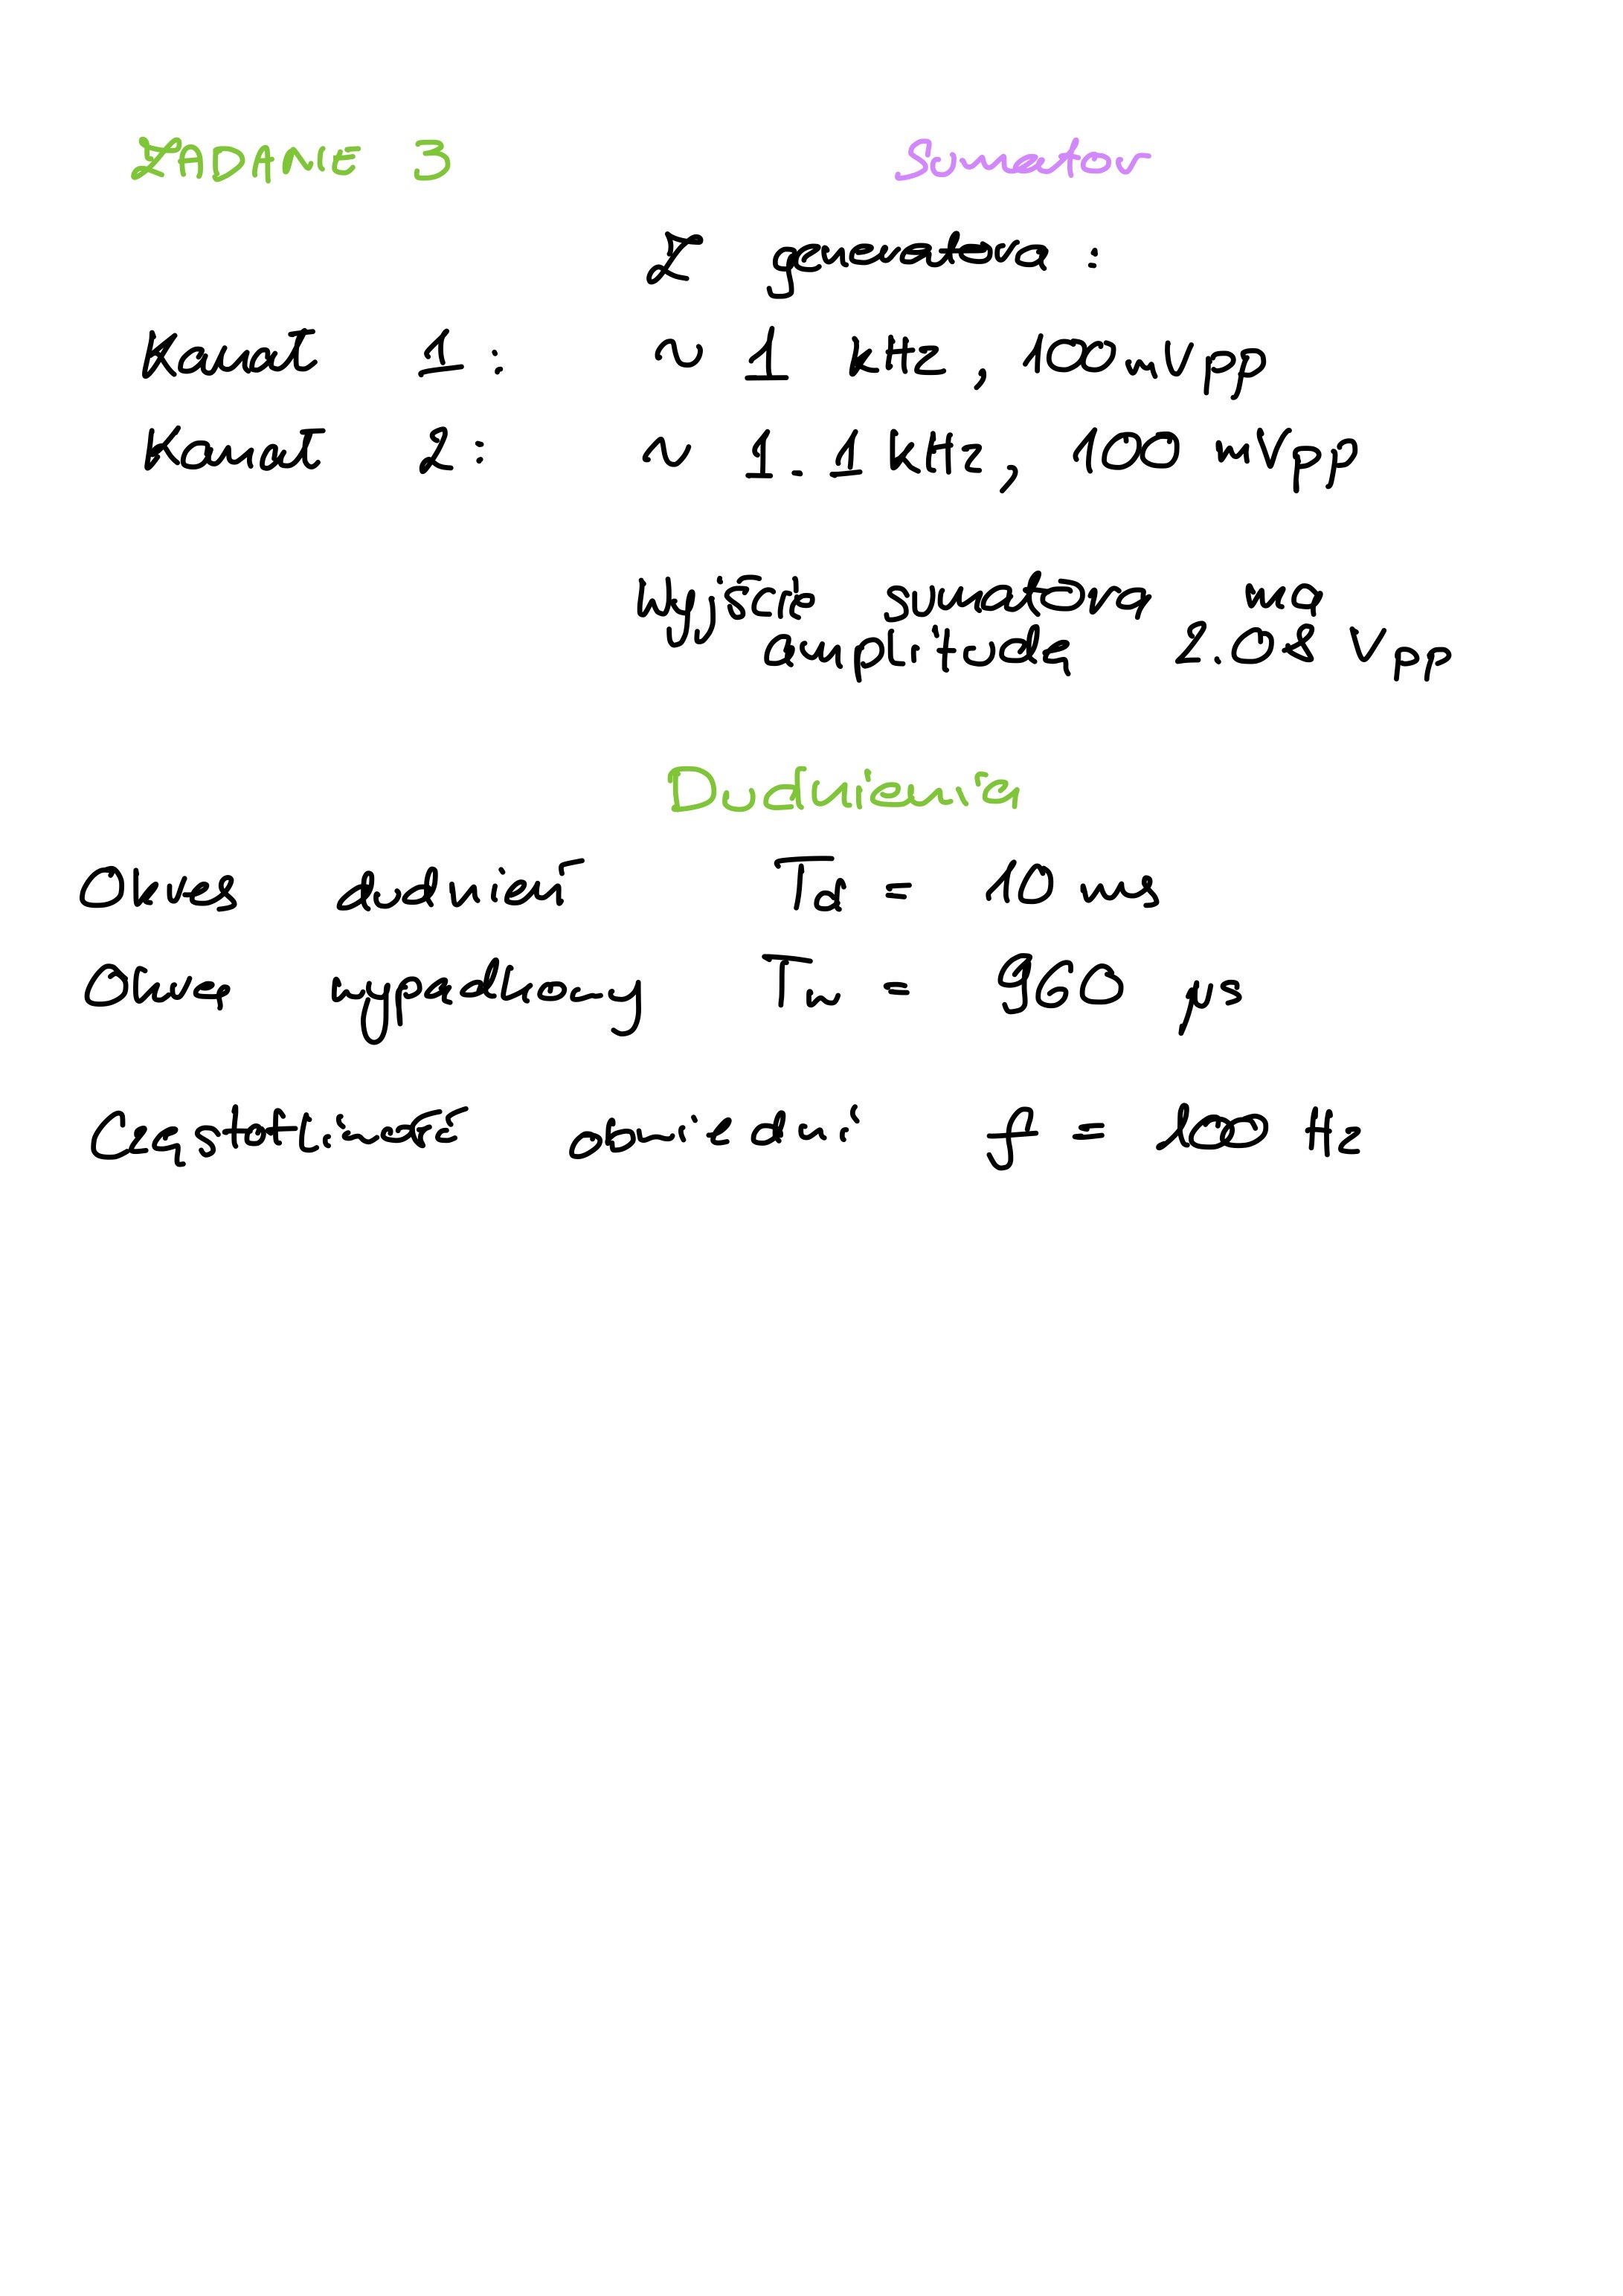
\includegraphics[scale=0.2]{B2}
\centering
\captionsetup{labelformat=empty}
\caption{}
\end{figure}

\begin{figure}[H]
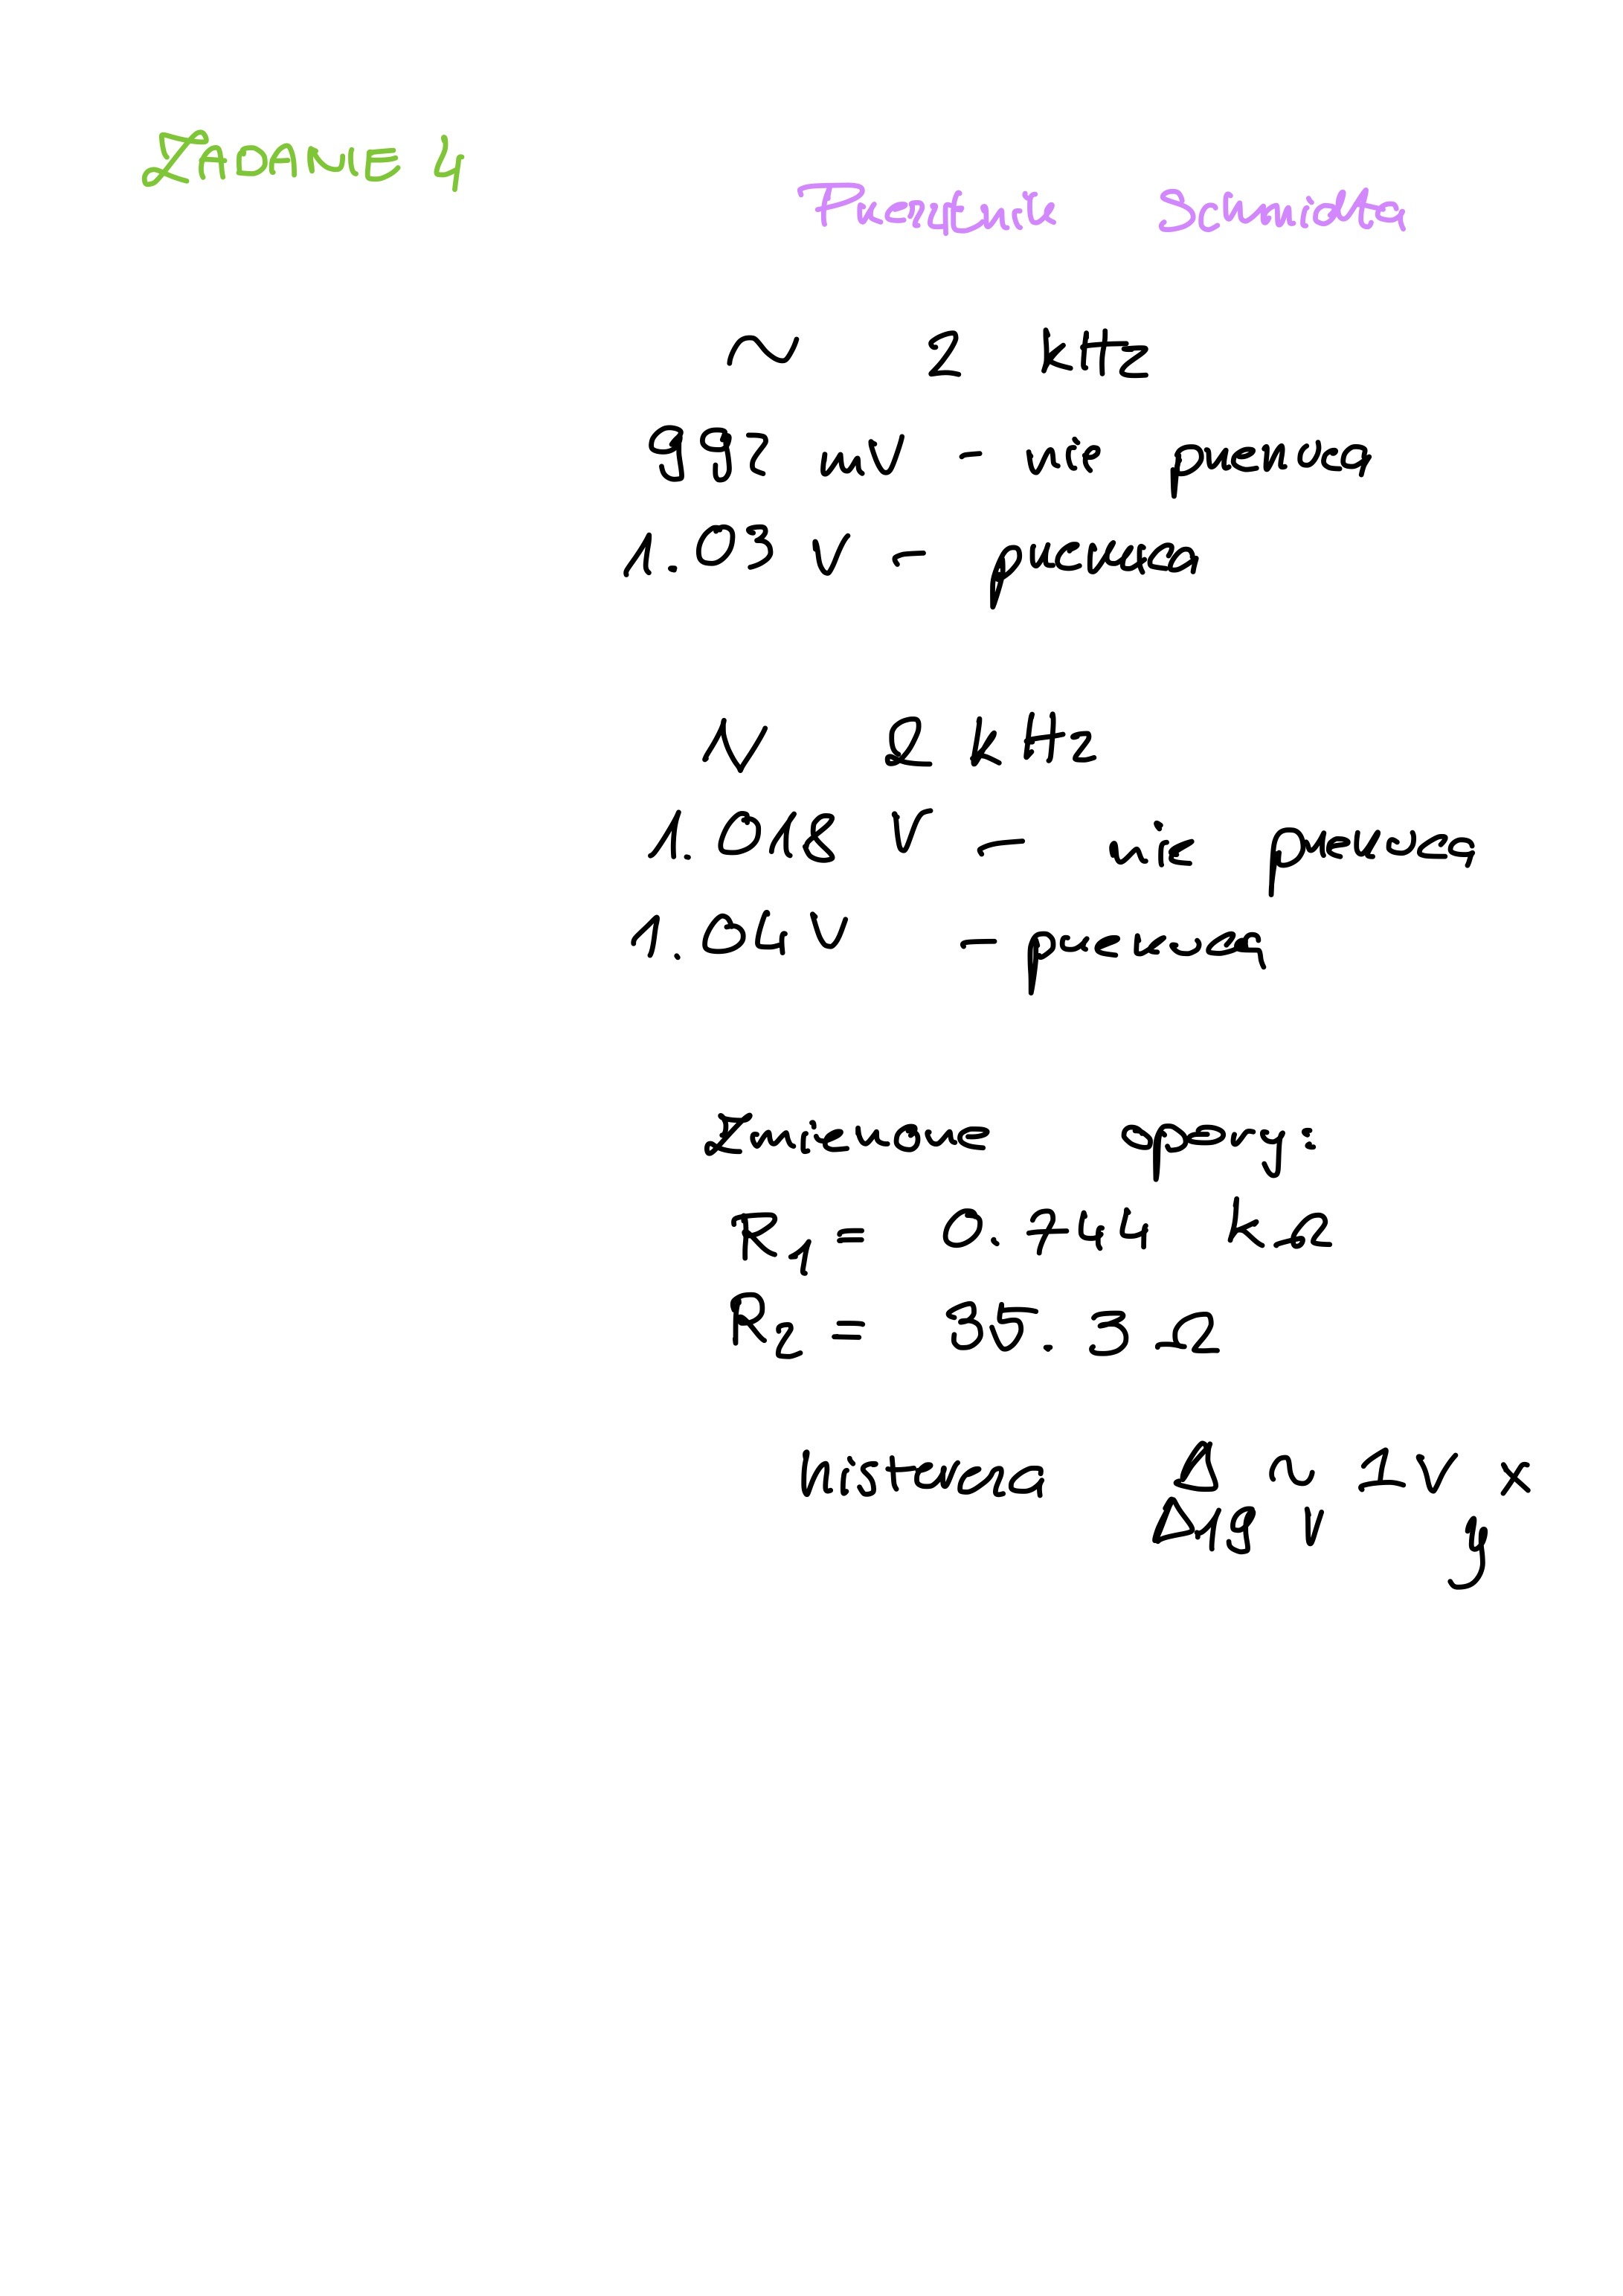
\includegraphics[scale=0.2]{B3}
\centering
\captionsetup{labelformat=empty}
\caption{}
\end{figure}

\begin{figure}[H]
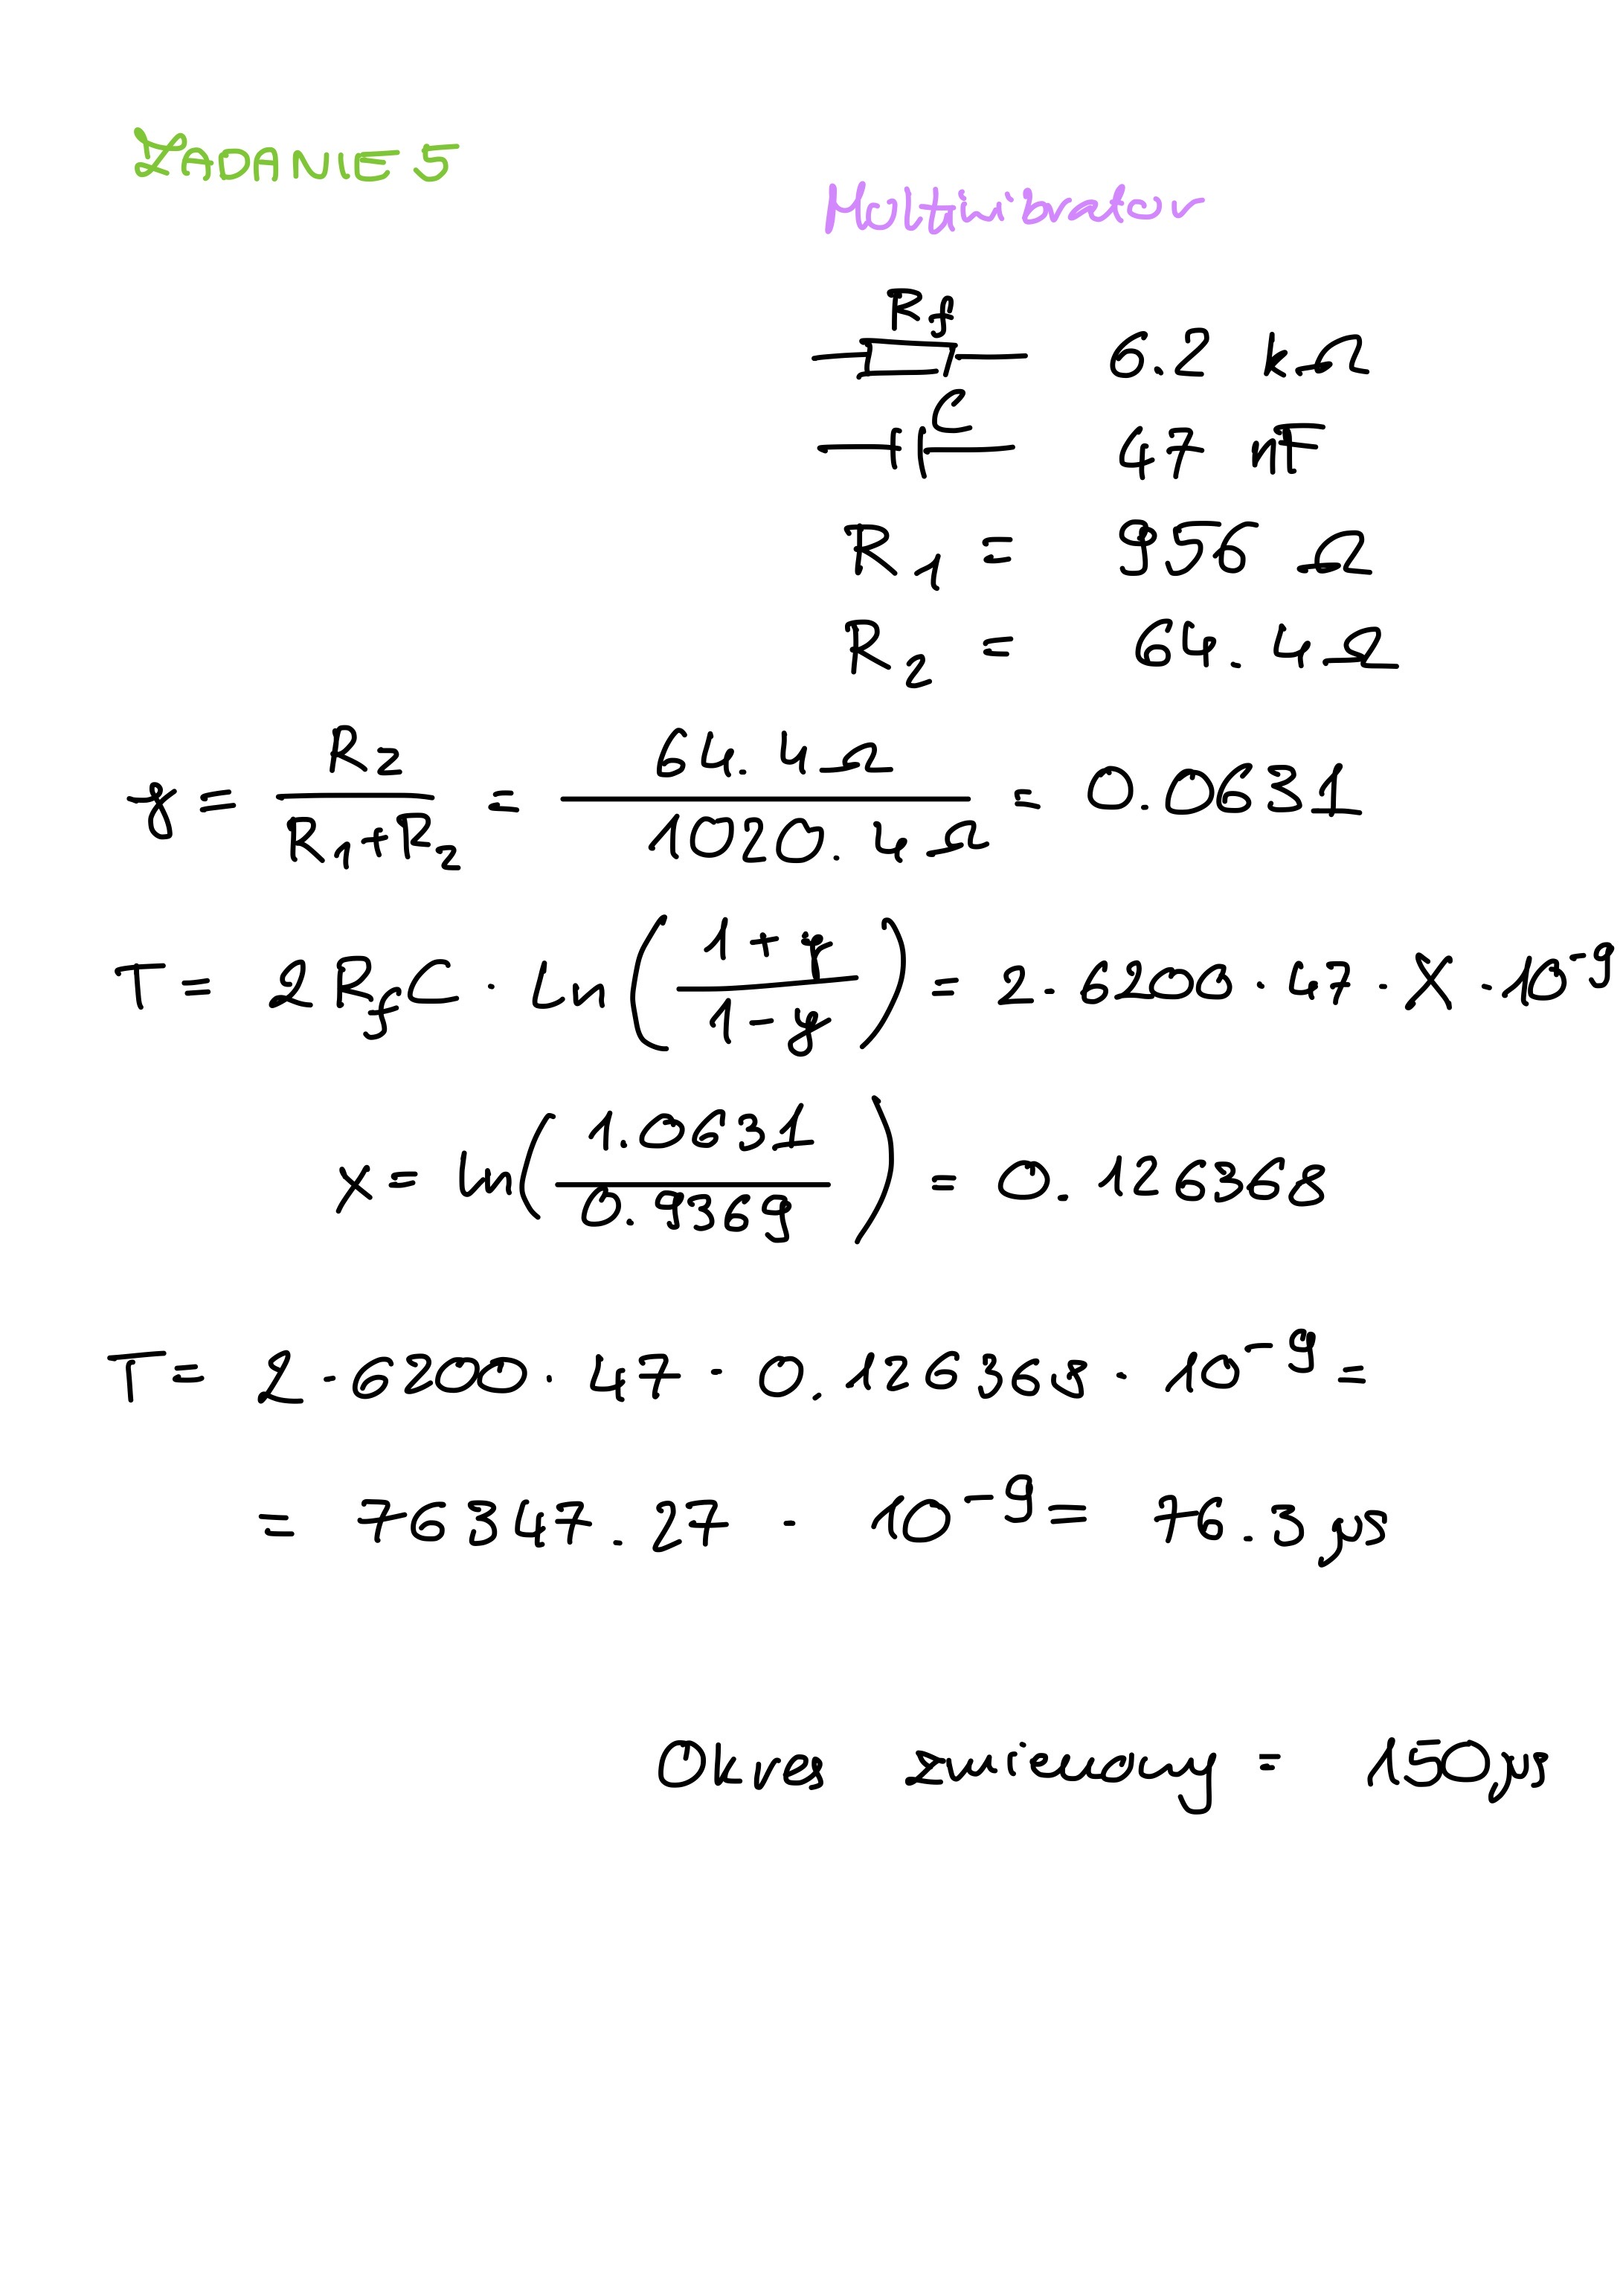
\includegraphics[scale=0.2]{B4}
\centering
\captionsetup{labelformat=empty}
\caption{}
\end{figure}

\end{document}
